\cleardoublepage
\chapter{Developer Documentation}
\label{ch:design}

This chapter documents the technical contribution of the thesis through
three implemented thesis contributions. The first contribution is an
OCR-based nutrition-label processing workflow that accepts uploaded
food-label images, extracts text, and converts the result into a
structured nutritional representation. The second contribution is a
structured recipe-generation and personalization workflow that combines
ingredient-based input, retrieval-augmented generation, and user
constraints such as dietary preferences and allergens. The third
contribution is the backend and persistence layer that integrates these
workflows into one application, supports authenticated use, and stores
user-specific data such as preferences, generated recipes, and OCR
history.

The rest of the chapter explains these contributions from three
perspectives. The design section presents the planned structure and
responsibilities of the system, the implementation section shows how
that design was realized in code, and the testing section evaluates the
resulting application behavior.

\cleardoublepage

\section{Design}
\label{sec:design}

This section presents the design of the \emph{AI Cookbook with
Ingredient-Based Search} system. The goal of the design is not to
repeat implementation details, but to explain how the system was
structured before discussing concrete modules and code in the later
implementation section. The design had to cover three core concerns of the project:
user-facing interaction, backend application logic, and persistent
data management.

The system solves two closely related problems. First, it helps users
generate recipes from available ingredients while respecting dietary
preferences and allergy constraints. Second, it extracts structured
nutrition data from food-label images so that the user does not need
to transcribe labels manually. These two features share the same
application shell, authentication model, and persistence layer, but
they differ in workflow shape: recipe generation is a retrieval- and
generation-oriented pipeline, while OCR is an image-processing and
information-extraction pipeline. The design therefore emphasizes clear
separation between routes, services, providers, and storage.

\subsection{Design Drivers and Requirements}

\subsubsection{Design goals and principles}

The design of the system is guided by a small set of principles that
reflect the actual risks and responsibilities of an AI-assisted cooking
application.

\begin{itemize}
	\item \textbf{Safety-oriented generation.} Allergy and dietary
	constraints should influence validation, retrieval, prompt
	construction, output checking, and warning generation instead of being
	treated as decorative metadata.
	\item \textbf{Explainability and transparency.} The system should make
	AI-supported decisions visible through warnings, excluded ingredients,
	raw OCR text, and structured nutrition output rather than hiding them
	behind a black-box interface.
	\item \textbf{Modularity.} Routes, services, providers, persistence
	models, and frontend task pages should remain separated by
	responsibility so that changes in one subsystem do not force unrelated
	rework elsewhere.
	\item \textbf{Reproducibility.} The application should be rebuildable
	from versioned source, migrations, dependency manifests, environment
	settings, and indexing scripts, which is important both for thesis
	evaluation and for repeatable local deployment.
	\item \textbf{User trust.} Users should be able to understand what was
	generated, what was inferred, and what limitations still apply. In
	this project, trust is built through predictable workflows and visible
	evidence rather than through stylistic polish alone.
\end{itemize}

These principles shape the rest of the design chapter. The requirements,
workflows, architecture, data model, and user interface all follow the
same priorities, so the chapter remains focused on one system instead
of reading as a set of separate technical topics.

\subsubsection{System purpose}

The application is designed as an interactive web system rather than a
single-run AI script. Users should be able to move between recipe
generation, OCR-based nutrition extraction, account management, and
history views through a stable browser interface. The backend is
responsible for validating requests, enforcing ownership rules,
orchestrating AI-supported workflows, and persisting user-specific
results.

From a design perspective, the most important objective is controlled
workflow execution. The application accepts user input that can be
unsafe or incomplete, and it also depends on external AI services that
may return imperfect outputs. For that reason, the design does not
treat generation as a single black-box API call. Instead, it introduces
validation, filtering, retrieval, output checking, optional retry, and
selective persistence as explicit stages.

\subsubsection{Primary actors and major use cases}

The system has two human-facing roles and one external-service role.

\begin{itemize}
	\item \textbf{Guest user.} Can generate recipes and run OCR
	extraction, but cannot persist private data.
	\item \textbf{Authenticated user.} Can use the guest-level functions
   and can also manage profile defaults, save recipes, and browse recipe
   and OCR history.
	\item \textbf{External AI services.} Provide text generation,
	embeddings, OCR text extraction, and recipe-image generation.
\end{itemize}

The main user-visible use cases are registration, login, profile
update, recipe generation, recipe saving, browsing saved recipes,
browsing recipe history, OCR extraction, and OCR result saving. The
table below lists only external actors; the backend itself is part of
the system and is discussed later in the architecture section.

\par\bigskip

\begin{table}[H]
	\centering
	\scriptsize
	\begin{tabular}{|p{3.1cm}|p{10.8cm}|}
		\hline
		\textbf{Actor} & \textbf{Responsibilities} \\
		\hline
		Guest user & Provides ingredients or nutrition-label images, triggers recipe generation and OCR extraction, reviews returned results, and explores the application without private persistence features. \\
		\hline
		Authenticated user & Owns guest capabilities and additionally manages stored profile defaults, saves generated recipes, browses recipe history, and persists OCR extraction history under a private account scope. \\
		\hline
		External AI services & Supply embeddings, recipe generation, recipe-thumbnail generation, and OCR text extraction through provider-facing interfaces used by the backend workflows. \\
		\hline
	\end{tabular}
	\caption{Actors and responsibilities in the AI Cookbook system}
	\label{tab:actors-responsibilities}
\end{table}

\begin{figure}[H]
	\centering
	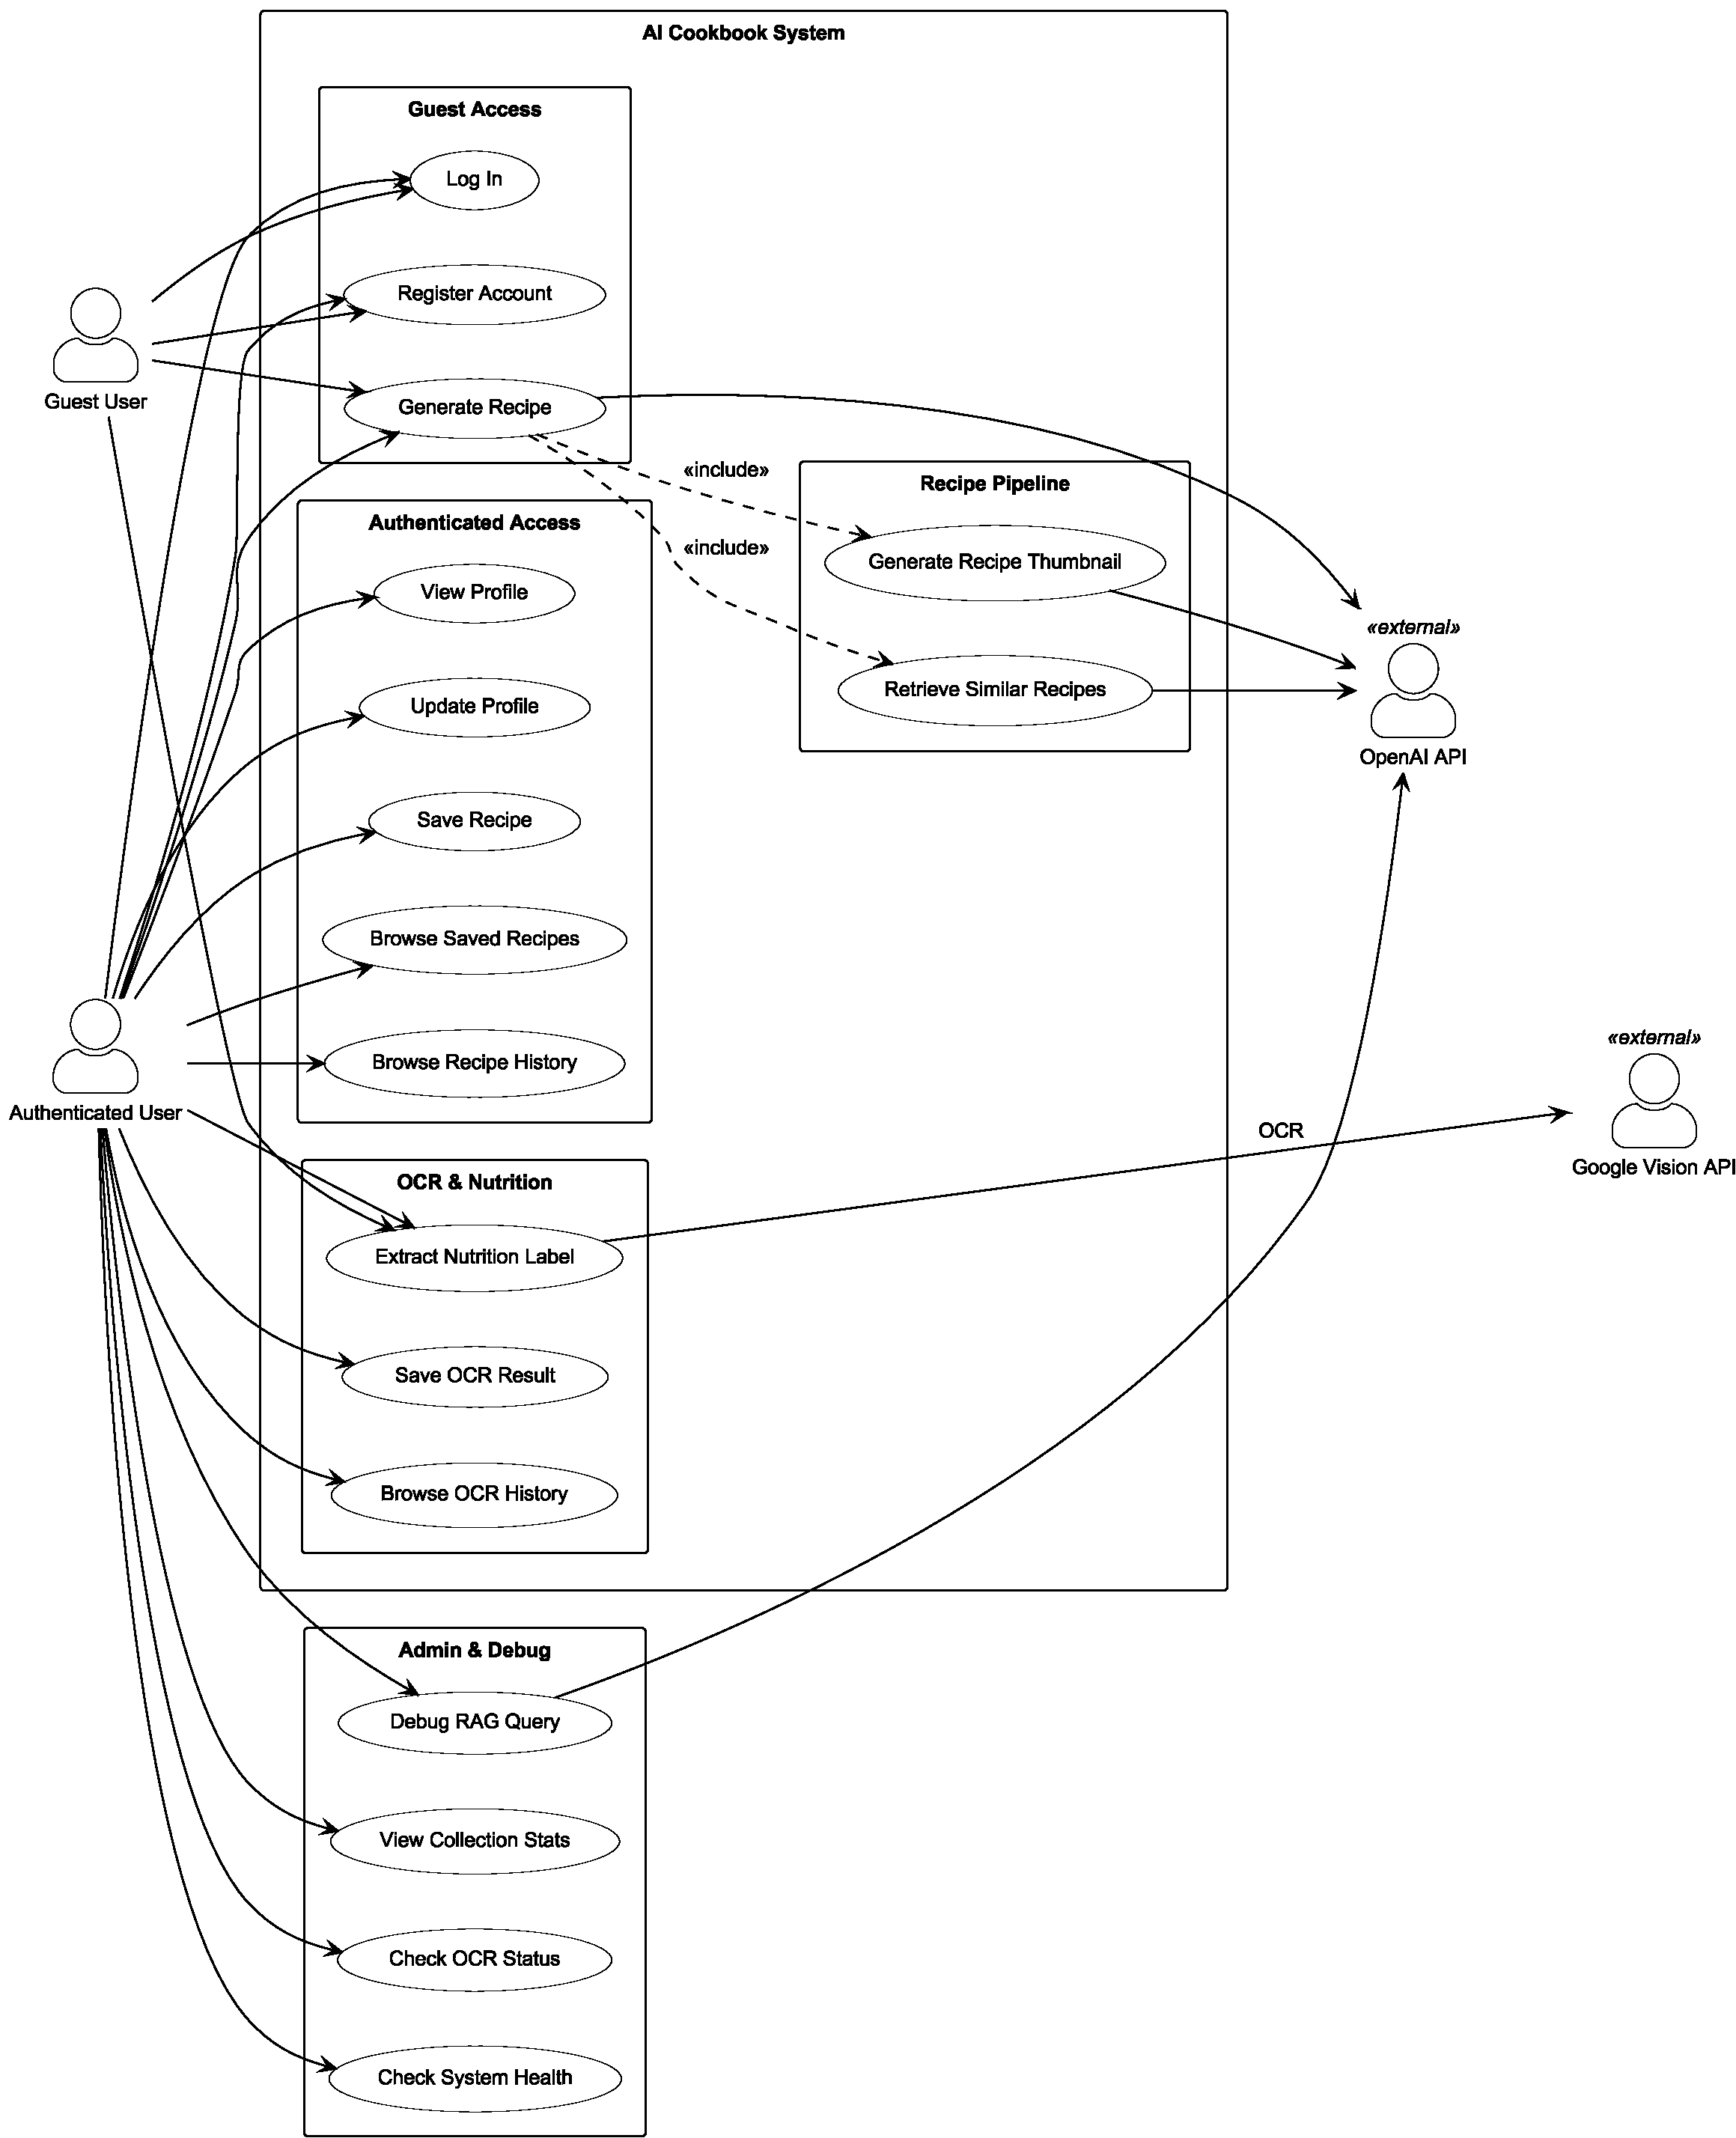
\includegraphics[width=\textwidth]{images/use-case-diagram.pdf}
	\caption{Use case diagram of the main user-visible system functions}
	\label{fig:design-use-case}
\end{figure}

\subsubsection{Functional requirements}

The main functional requirements of the system are the following.

\begin{enumerate}
	\item \textbf{FR-1: Ingredient-based recipe generation.} The system
	shall accept a non-empty ingredient list and return a structured
	recipe containing a title, ingredient list, preparation steps, and a
	nutrition estimate.
	\item \textbf{FR-2: Preference- and allergy-aware generation.} The
	system shall allow the request to include dietary preferences and
	allergy constraints, and these constraints shall influence the recipe
	generation workflow.
	\item \textbf{FR-3: Retrieval-grounded generation.} Before recipe
	generation, the system shall retrieve relevant recipe context from an
	indexed recipe corpus and use that context to ground the language
	model.
	\item \textbf{FR-4: User authentication.} The system shall support
	user registration, login, and retrieval of the current authenticated
	profile.
	\item \textbf{FR-5: Profile defaults.} The system shall allow
	authenticated users to store dietary preferences and allergies as
	profile defaults.
	\item \textbf{FR-6: Recipe history.} The system shall persist generated
	recipes for authenticated users and make them available through a
	history view.
	\item \textbf{FR-7: Explicit recipe saving.} The system shall allow an
	authenticated user to mark a generated recipe as saved and display
	saved recipes separately from full history.
	\item \textbf{FR-8: OCR extraction.} The system shall accept a food
	label image, validate it, extract raw text, and return structured
	nutrition fields.
	\item \textbf{FR-9: OCR history.} The system shall allow authenticated
	users to save OCR results and later browse those extractions through a
	history view.
	\item \textbf{FR-10: Protected ownership.} The system shall ensure that
	saved recipes, generation history, OCR history, and profile data are
	visible only to the owning authenticated user.
\end{enumerate}

The design makes these requirements testable through explicit input
limits, response-shape guarantees, and route behavior. Those measurable
criteria are summarized in Table~\ref{tab:design-fr-criteria}.

\begin{table}[H]
	\centering
	\scriptsize
	\begin{tabular}{|p{1.4cm}|p{5.7cm}|p{7.2cm}|}
		\hline
		\textbf{ID} & \textbf{Requirement focus} & \textbf{Acceptance criterion derived from the design} \\
		\hline
		FR-1 & Recipe request and response structure & A recipe request contains 1--25 ingredients; each ingredient string is at most 80 characters after trimming. A successful response contains a title, ingredient list, step list, and nutrition estimate object. \\
		\hline
		FR-2 & Constraint-aware generation & Preference and allergy lists may each contain at most 10 entries. Ingredients conflicting with declared allergies or dietary preferences are excluded before generation and surfaced as warnings in the response. \\
		\hline
		FR-3 & Retrieval grounding & For every recipe request, the backend queries the vector store for up to 10 candidates, filters unsafe matches, ranks the remainder, and forwards the best 3 contexts to the generation prompt. \\
		\hline
		FR-4 & Authentication lifecycle & The system exposes dedicated signup, login/token, and current-user profile retrieval routes. Passwords are never stored in plaintext, and authenticated identity is reconstructed from a signed JWT. \\
		\hline
		FR-5 & Profile defaults & The authenticated user can persist default preferences and allergies, and those values are returned as part of the profile representation. \\
		\hline
		FR-6 & Recipe history & When the requester is authenticated, every successful recipe generation creates a history row owned by that user. History listing is paginated with page size in the range 1--50. \\
		\hline
		FR-7 & Explicit saving & Saving a recipe requires authentication and a valid \texttt{generated\_recipe\_id} owned by the current user. The operation sets \texttt{is\_saved} and records \texttt{saved\_at}. \\
		\hline
		FR-8 & OCR extraction pipeline & OCR upload accepts common image formats, rejects empty uploads, enforces a maximum size of 5\,242\,880 bytes and a maximum of 20\,000\,000 pixels, then returns both raw OCR text and structured nutrition fields. \\
		\hline
		FR-9 & OCR history & Saved OCR results are persisted only for authenticated users and listed through a paginated history endpoint with page size in the range 1--50. \\
		\hline
		FR-10 & Ownership protection & Recipe save/list/history and OCR save/history queries are always filtered by the authenticated user identifier, so one user's records are not visible to another. \\
		\hline
	\end{tabular}
	\caption{Measurable acceptance criteria for the functional requirements}
	\label{tab:design-fr-criteria}
\end{table}

\subsubsection{Non-functional requirements}

The design also had to satisfy several non-functional requirements.

\begin{enumerate}
	\item \textbf{NFR-1: Usability.} The main workflows should be
	discoverable through a small and stable set of pages.
	\item \textbf{NFR-2: Safety-oriented behavior.} The recipe-generation
	workflow should explicitly consider allergies and dietary preferences
	rather than treating them as informational metadata only.
	\item \textbf{NFR-3: Maintainability.} The system should separate
	presentation logic, request handling, service orchestration,
	persistence, and external-provider integration.
	\item \textbf{NFR-4: Reproducibility.} A new local environment should
	be able to run the system from declared dependencies, environment
	configuration, migration files, and indexing scripts.
	\item \textbf{NFR-5: Basic security.} The design should include
	password hashing, token-based authentication, user-scoped data access,
	and route-level rate limiting.
	\item \textbf{NFR-6: Thesis-scale performance.} The system should
	remain responsive for ordinary interactive use with a moderate local
	vector index and paginated history access.
\end{enumerate}

Table~\ref{tab:design-nfr-criteria} translates these quality goals into
concrete design targets that can be checked against the implemented
system.

\begin{table}[H]
	\centering
	\scriptsize
	\begin{tabular}{|p{1.4cm}|p{5.7cm}|p{7.2cm}|}
		\hline
		\textbf{ID} & \textbf{Quality goal} & \textbf{Concrete design target} \\
		\hline
		NFR-1 & Usability & Top-level navigation is limited to six stable routes: Home, Generate, Food Labels, Saved, History, and Login/Account. Each major user task has a dedicated page rather than a shared overloaded view. \\
		\hline
		NFR-2 & Safety-oriented behavior & Conflicting input ingredients are removed before prompt construction, unsafe generated outputs are checked against restriction keywords, and the recipe workflow may issue one corrective retry before failing. \\
		\hline
		NFR-3 & Maintainability & Route handlers do not call provider SDKs directly. External OCR, image generation, embeddings, and LLM calls are isolated behind service or provider modules. API schemas are separated from ORM entities. \\
		\hline
		NFR-4 & Reproducibility & Backend configuration is centralized in environment-backed settings, relational changes are represented through migration files, and recipe-corpus preparation plus vector indexing are scriptable offline steps. \\
		\hline
		NFR-5 & Security & Passwords are hashed with a dedicated password-hashing library, access tokens expire after 60 minutes, and route-specific rate limits are enforced: 5 requests / 15 minutes for auth routes, 15 / 15 minutes for recipe generation, and 10 / 15 minutes for OCR extraction. \\
		\hline
		NFR-6 & Thesis-scale performance & Saved and history queries are paginated with page size capped at 50. Retrieval is bounded to 10 vector candidates and 3 final context items, limiting per-request downstream prompt size. \\
		\hline
	\end{tabular}
	\caption{Concrete design targets for the non-functional requirements}
	\label{tab:design-nfr-criteria}
\end{table}

\subsubsection{Narrative use-case descriptions}

The use-case diagram in Figure~\ref{fig:design-use-case} shows the full
actor-function landscape. The following three narrative descriptions
focus on the workflows that shape the system design most strongly.

\paragraph{UC-1: Generate a recipe from ingredients.}
\textbf{Primary actor:} Guest user or authenticated user. \\
\textbf{Preconditions:} The user opens the Generate page and provides at
least one non-blank ingredient. Optional dietary preferences and
allergies may also be provided directly or inherited from the profile
defaults of an authenticated user. \\
\textbf{Main success scenario:}
\begin{enumerate}
	\item The user submits a recipe-generation request.
	\item The backend validates the request structure and trims the string
	values.
	\item The workflow removes ingredients that conflict with declared
	allergies or dietary preferences.
	\item The system retrieves relevant safe recipe context from the vector
	store and builds a grounded generation prompt.
	\item The language model returns a structured recipe, which is checked
	for restriction violations and supplemented with warnings if needed.
	\item The system attempts to generate a thumbnail image.
	\item If the user is authenticated, the generated recipe is stored in
	the recipe-history table.
	\item The user receives the final recipe, optional warnings, and the
	thumbnail if image generation succeeded.
\end{enumerate}
\textbf{Alternative flows:}
\begin{enumerate}
	\item If every provided ingredient conflicts with the declared
	constraints, the request is rejected with a validation-style error and
	no generation is attempted.
	\item If the first model output still violates the restrictions, a
	corrective retry is executed once.
	\item If thumbnail generation fails, the recipe is still returned, but
	a warning is attached and the response contains no image URL.
\end{enumerate}
\textbf{Postconditions:} A structured recipe has been delivered. If the
requester was authenticated, the unsaved generated result exists in the
history table and can later be explicitly saved.

\paragraph{UC-2: Save a generated recipe.}
\textbf{Primary actor:} Authenticated user. \\
\textbf{Preconditions:} The user is logged in and already owns a
generated recipe entry created by the recipe-generation workflow. \\
\textbf{Main success scenario:}
\begin{enumerate}
	\item The user selects the Save action on a generated recipe.
	\item The frontend sends the stored \texttt{generated\_recipe\_id} to
	the backend.
	\item The backend verifies that the referenced recipe belongs to the
	current authenticated user.
	\item The system marks the recipe as saved and records the save
	timestamp.
	\item The saved-recipes view becomes able to display the entry
	separately from full history.
\end{enumerate}
\textbf{Alternative flow:} If the identifier does not exist or belongs
to another user, the save request is rejected with a not-found response. \\
\textbf{Postconditions:} The recipe remains in history and is also
visible through the saved-recipes listing.

\paragraph{UC-3: Extract structured nutrition data from a food label.}
\textbf{Primary actor:} Guest user or authenticated user. \\
\textbf{Preconditions:} The user selects an image file in a supported
format and the upload satisfies the configured size and pixel limits. \\
\textbf{Main success scenario:}
\begin{enumerate}
	\item The user uploads a nutrition-label image from the Food Labels
	page.
	\item The backend validates file type, non-emptiness, size, and image
	dimensions.
	\item The system attempts to store the upload in the
	backend-managed media directory before OCR processing continues.
	\item The image is preprocessed for OCR and forwarded to the OCR
	provider.
	\item The raw OCR text is returned and then converted into a fixed
	nutrition JSON structure.
	\item The user sees both the raw extracted text and the structured
	nutrition fields.
	\item If the user is authenticated and chooses to save the result, the
	extraction is persisted to the OCR history table.
\end{enumerate}
\textbf{Alternative flows:}
\begin{enumerate}
	\item If the uploaded file is empty or exceeds the configured limits,
	the request is rejected before provider calls are made.
	\item If OCR succeeds but nutrition structuring fails, the backend
	rejects the request because the workflow requires a complete
	structured nutrition result.
\end{enumerate}
\textbf{Postconditions:} The user receives either a validated nutrition
payload or a clear failure response. Authenticated users may persist the
result for later review.

\subsection{Architecture and System Design}

\subsubsection{Architectural style}

The system follows a layered client--server architecture. The frontend
is responsible for presentation, route navigation, and local
interaction state. The backend exposes an HTTP API for validation,
authentication, persistence, and orchestration of the AI workflows.
Storage is split across three backend-managed layers: a relational
database, a vector store, and the local filesystem for media assets.

This structure follows directly from what the application has to do.
User-scoped history persistence, OCR validation and preprocessing,
retrieval from the recipe corpus, prompt construction, and provider
calls all belong on the backend side. The browser mainly handles forms,
navigation, conditional rendering, and result presentation. Keeping
these responsibilities separate makes the main workflows easier to
control and easier to extend.

\subsubsection{Layered architecture}

The layered style is the main organizational rule of the system. The
browser layer is responsible for forms, navigation, local interaction
state, and result presentation. It does not validate business
constraints beyond basic user-interface checks, and it never
communicates directly with the relational database, vector store,
filesystem, or provider SDKs.

The backend API layer serves as the controlled entry point into the
system. Route modules receive JSON requests, validate them through
schemas, resolve authentication state, and delegate non-trivial work to
the service layer. The service layer then coordinates recipe
generation, OCR processing, retrieval, image generation, and response
assembly in a fixed order. Below that, the storage and provider layers
separate persistent state from external integrations: relational tables
store user-owned data, the vector store supports retrieval, the local
filesystem stores media, and provider adapters isolate third-party API
details.

This layering is especially important because the system combines
ordinary web-application responsibilities with AI-assisted workflows.
Without explicit layers, validation, persistence, provider logic, and
result presentation would quickly become entangled.

\subsubsection{Architectural decomposition rationale}

The structural decomposition of the system follows directly from the two
main workflows introduced earlier. Recipe generation requires a
request--validation boundary, a retrieval subsystem, a generation
orchestration layer, persistence for user-owned history, and optional
media generation. OCR-based nutrition extraction requires an upload
boundary, image preprocessing, provider-facing extraction logic,
semantic structuring of the extracted text, and optional persistence of
results. These workflows share authentication, ownership control, and
the browser-facing navigation shell, but they differ enough internally
that they are kept as separate backend modules.

This decomposition also keeps later changes manageable. The frontend is
limited to page interaction and result presentation. The backend
controls validation, workflow order, and access rules. Persistent state
is split into relational data, retrieval data, and media assets.
Provider-specific behavior is kept behind separate boundaries, so
changes in OCR or image generation do not ripple through the user-facing
API or the persistence model.

\subsubsection{High-level component model}

At the highest level, the system is decomposed into the following
components:

\begin{itemize}
	\item \textbf{Single-page frontend} for user-facing pages and interaction.
	\item \textbf{Backend API layer} for request routing and workflow
	orchestration.
	\item \textbf{Authentication/profile module} for user identity and
	default constraints.
	\item \textbf{Recipe-generation module} for RAG-based recipe creation
	and recipe persistence.
	\item \textbf{OCR module} for label-image processing and nutrition
	structuring.
	\item \textbf{Relational database} for transactional persistence.
	\item \textbf{Vector store} for retrieval support.
	\item \textbf{Filesystem media storage} for OCR uploads and generated
	thumbnails.
	\item \textbf{External AI providers} for OCR, text generation,
	embeddings, and image generation.
\end{itemize}

\begin{figure}[H]
	\centering
	\resizebox{\textwidth}{!}{
	\begin{tikzpicture}[
		comp/.style={draw, rounded corners, minimum width=3.2cm, minimum height=1.1cm, align=center},
		store/.style={draw, cylinder, shape border rotate=90, aspect=0.25, minimum height=1.2cm, minimum width=2.1cm, align=center},
		ext/.style={draw, rounded corners, dashed, minimum width=3.0cm, minimum height=1.0cm, align=center},
		>=Latex
	]
	\node[comp] (frontend) at (0,5.6) {Frontend};
	\node[comp] (backend) at (0,3.7) {Backend API};

	\node[comp] (auth) at (-5.0,1.8) {Auth \& profile\\module};
	\node[comp] (recipes) at (-1.7,1.8) {Recipe-generation\\module};
	\node[comp] (ocr) at (1.7,1.8) {OCR\\module};
	\node[comp] (media) at (5.0,1.8) {Media\\serving};

	\node[store] (db) at (-4.3,-0.4) {Relational DB};
	\node[store] (chroma) at (-1.1,-0.4) {Vector store};
	\node[store] (files) at (2.1,-0.4) {Media files};
	\node[ext] (openai) at (5.3,-0.4) {OpenAI APIs};
	\node[ext] (vision) at (5.3,-2.0) {Google Vision API};

	\draw[-Latex] (frontend) -- node[right] {HTTP/JSON} (backend);

	\draw[-Latex] (backend) -- (auth);
	\draw[-Latex] (backend) -- (recipes);
	\draw[-Latex] (backend) -- (ocr);
	\draw[-Latex] (backend) -- (media);

	\draw[-Latex] (auth) -- (db);
	\draw[-Latex] (recipes) -- (db);
	\draw[-Latex] (recipes) -- (chroma);
	\draw[-Latex] (recipes) -- (files);
	\draw[-Latex] (recipes) -- (openai);
	\draw[-Latex] (ocr) -- (files);
	\draw[-Latex] (ocr) -- (vision);
	\draw[-Latex] (ocr) -- (openai);
	\draw[-Latex] (media) -- (files);
	\end{tikzpicture}}
	\caption{Component diagram of the system architecture}
	\label{fig:design-component}
\end{figure}

The component model also makes the layer boundaries visible. The
frontend never accesses the relational database, vector store, or
provider APIs directly. It talks only to the backend API. Within the backend, route modules remain
thin and delegate non-trivial work to services, providers, and storage
abstractions. This same decomposition reappears in the more detailed UML
artifacts presented next.

\begin{table}[H]
	\centering
	\scriptsize
	\renewcommand{\arraystretch}{1.2}
	\begin{tabularx}{\textwidth}{|p{2.8cm}|p{4.4cm}|X|}
		\hline
		\textbf{Layer} & \textbf{Implemented units} & \textbf{Primary responsibility} \\
		\hline
		Frontend interaction layer & React pages, navigation shell, shared auth context, reusable presentation components & Collect user input, maintain page-level interaction state, invoke backend routes, and render generated or retrieved results. \\
		\hline
		API boundary & FastAPI route modules and Pydantic request/response schemas & Validate request shape, enforce authentication or ownership checks, and expose a stable JSON contract to the browser. \\
		\hline
		Workflow and orchestration layer & Recipe-generation, OCR, retrieval, and image services & Execute multi-step application logic in a fixed order and isolate external-provider interactions from route handlers. \\
		\hline
		Provider integration layer & OCR and image-provider abstractions plus concrete adapters & Hide vendor-specific SDK calls behind application-facing interfaces such as \texttt{extract\_text()} and \texttt{generate\_png()}. \\
		\hline
		Transactional persistence layer & SQLAlchemy entities, database session handling, Alembic migrations & Store user accounts, generated recipes, OCR history, ownership relations, and pagination-supporting indexes. \\
		\hline
		Retrieval and media layer & Chroma vector store, recipe-indexing scripts, filesystem media storage & Persist retrieval documents and embeddings, store OCR uploads and thumbnails, and serve media files back to the frontend. \\
		\hline
	\end{tabularx}
\caption{Layer responsibilities in the implemented system}
	\label{tab:layer-responsibilities}
\end{table}

\subsubsection{Technology selection rationale}

The selected technologies follow the needs of the implemented
architecture instead of being chosen as a generic full-stack template.
The frontend is built as a React single-page application because the
main user tasks---recipe generation, OCR extraction, saved results, and
history browsing---share one navigation shell but require different
forms, loading states, and result layouts. A page-oriented React
frontend keeps those task flows separate while still allowing shared
authentication state and reusable result components.

The backend is built with FastAPI because the application depends on
clear request validation and on keeping route handlers thin. Recipe
generation, OCR extraction, save operations, and history listing all
accept structured input and return structured output, so schema-based
request and response handling fits the project well. This is especially
useful in the recipe workflow, where ingredient lists, allergies,
preferences, warnings, and nutrition fields all have to remain
well-formed across several processing stages.

Relational persistence is handled through SQLAlchemy with migration
support, because the project stores ownership-sensitive data rather than
anonymous prompt logs. User accounts, generated recipes, save state, and
OCR history need stable identifiers, foreign-key relationships, and
queryable timestamps. These requirements match a relational model more
closely than a document-only store.

The retrieval layer uses a persistent vector store because recipe
generation is grounded in a local recipe corpus. The system does not use
retrieval as an optional enhancement; it depends on retrieval to supply
context before prompt construction. For that reason, embeddings and
similarity search are treated as part of the architecture itself.

Media files are stored on the local filesystem because OCR uploads and
generated thumbnails act as supporting assets around the main
application data. The project needs these files to be saved, reused, and
served back to the frontend, but it does not need cloud-scale media
infrastructure for the bachelor-thesis scope. External AI providers are
used only where the project needs capabilities that are not implemented
locally, namely text generation, embeddings, OCR, and thumbnail
generation.

\subsubsection{Object-oriented modelling artifacts}

Although part of the backend is implemented in a function-oriented
style, the system still has a meaningful object-oriented structure. The
most important implemented classes fall into three groups:

\begin{itemize}
	\item \textbf{Persistent domain classes}, such as \texttt{User},
	\texttt{GeneratedRecipe}, and \texttt{OcrExtraction}.
	\item \textbf{Schema/data-transfer classes}, such as request and
	response models used at API boundaries.
	\item \textbf{Provider abstraction classes}, such as
	\texttt{OcrProvider}, \texttt{GoogleVisionOcrProvider},
	\texttt{RecipeImageProvider}, and
	\texttt{OpenAIRecipeImageProvider}.
\end{itemize}

The following class diagrams expand the earlier component view into the
implemented backend structures. The overview is split into two figures
to keep the diagrams readable at thesis page scale: one diagram focuses
on domain classes, provider abstractions, and the module-level service
boundaries around them, while the other focuses on schemas,
configuration, and infrastructure support.

\begin{figure}[htbp]
	\centering
	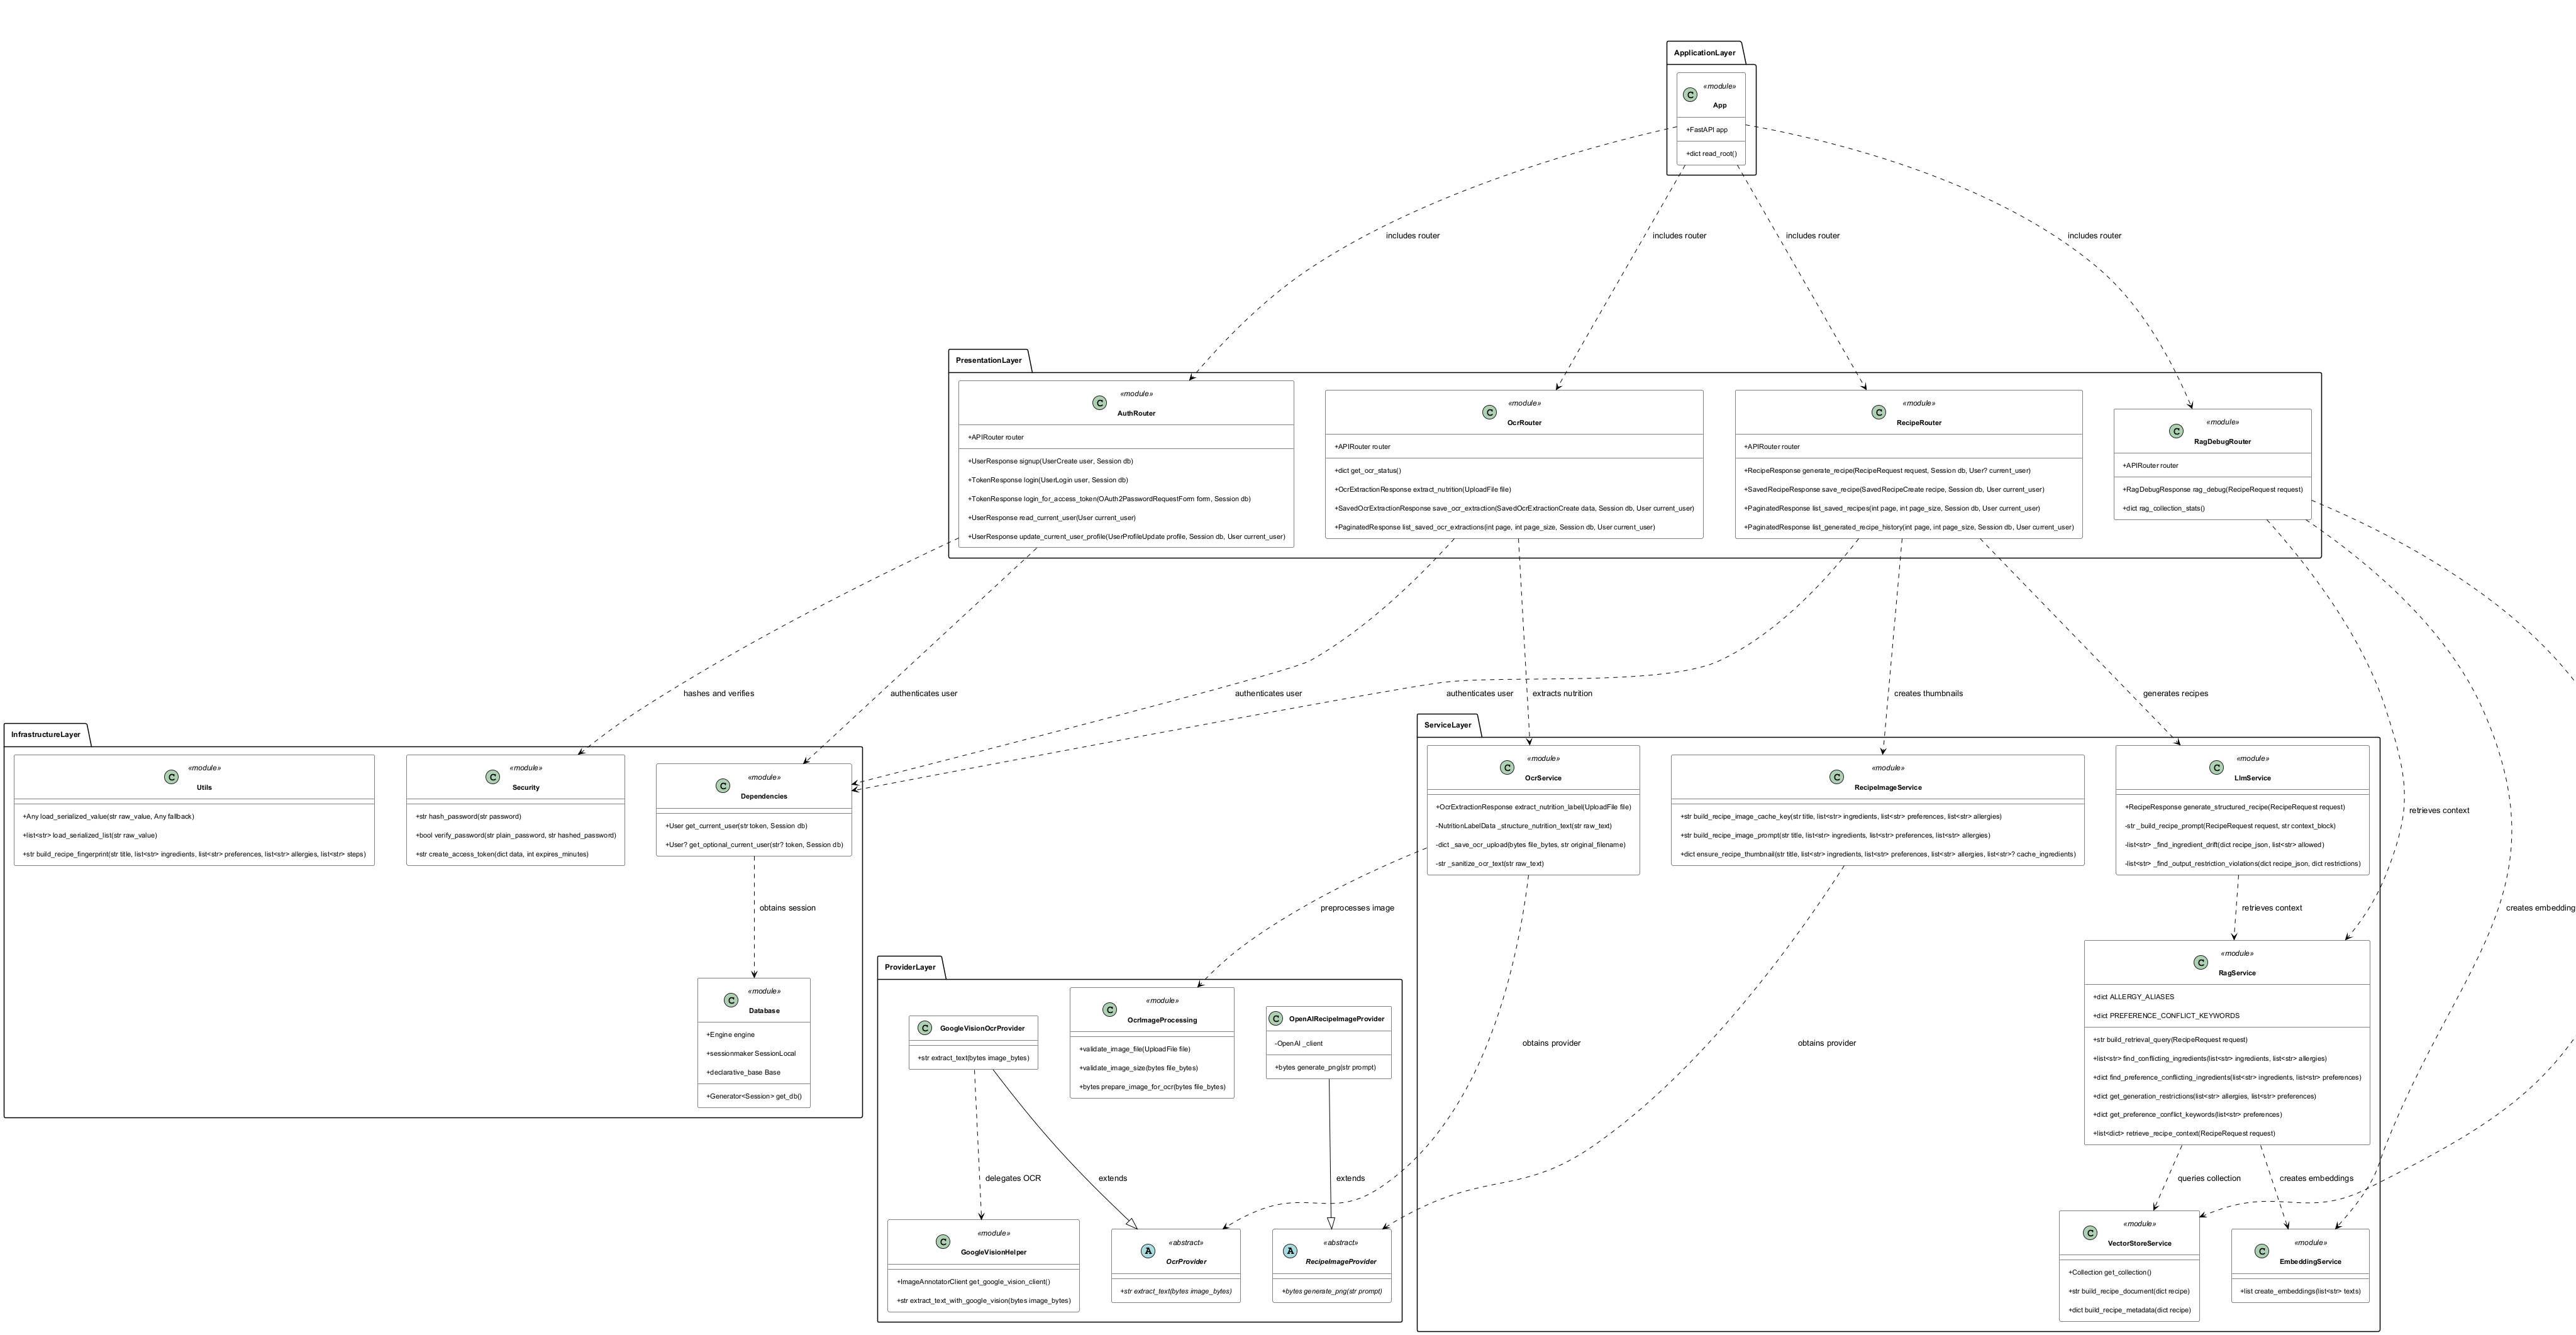
\includegraphics[width=\textwidth]{images/class-diagram-a.png}
	\caption{Class diagram of the domain and backend-service
	structure, showing implemented entity classes, provider
	abstractions, and their relationships}
	\label{fig:class-domain}
\end{figure}

\begin{figure}[htbp]
	\centering
	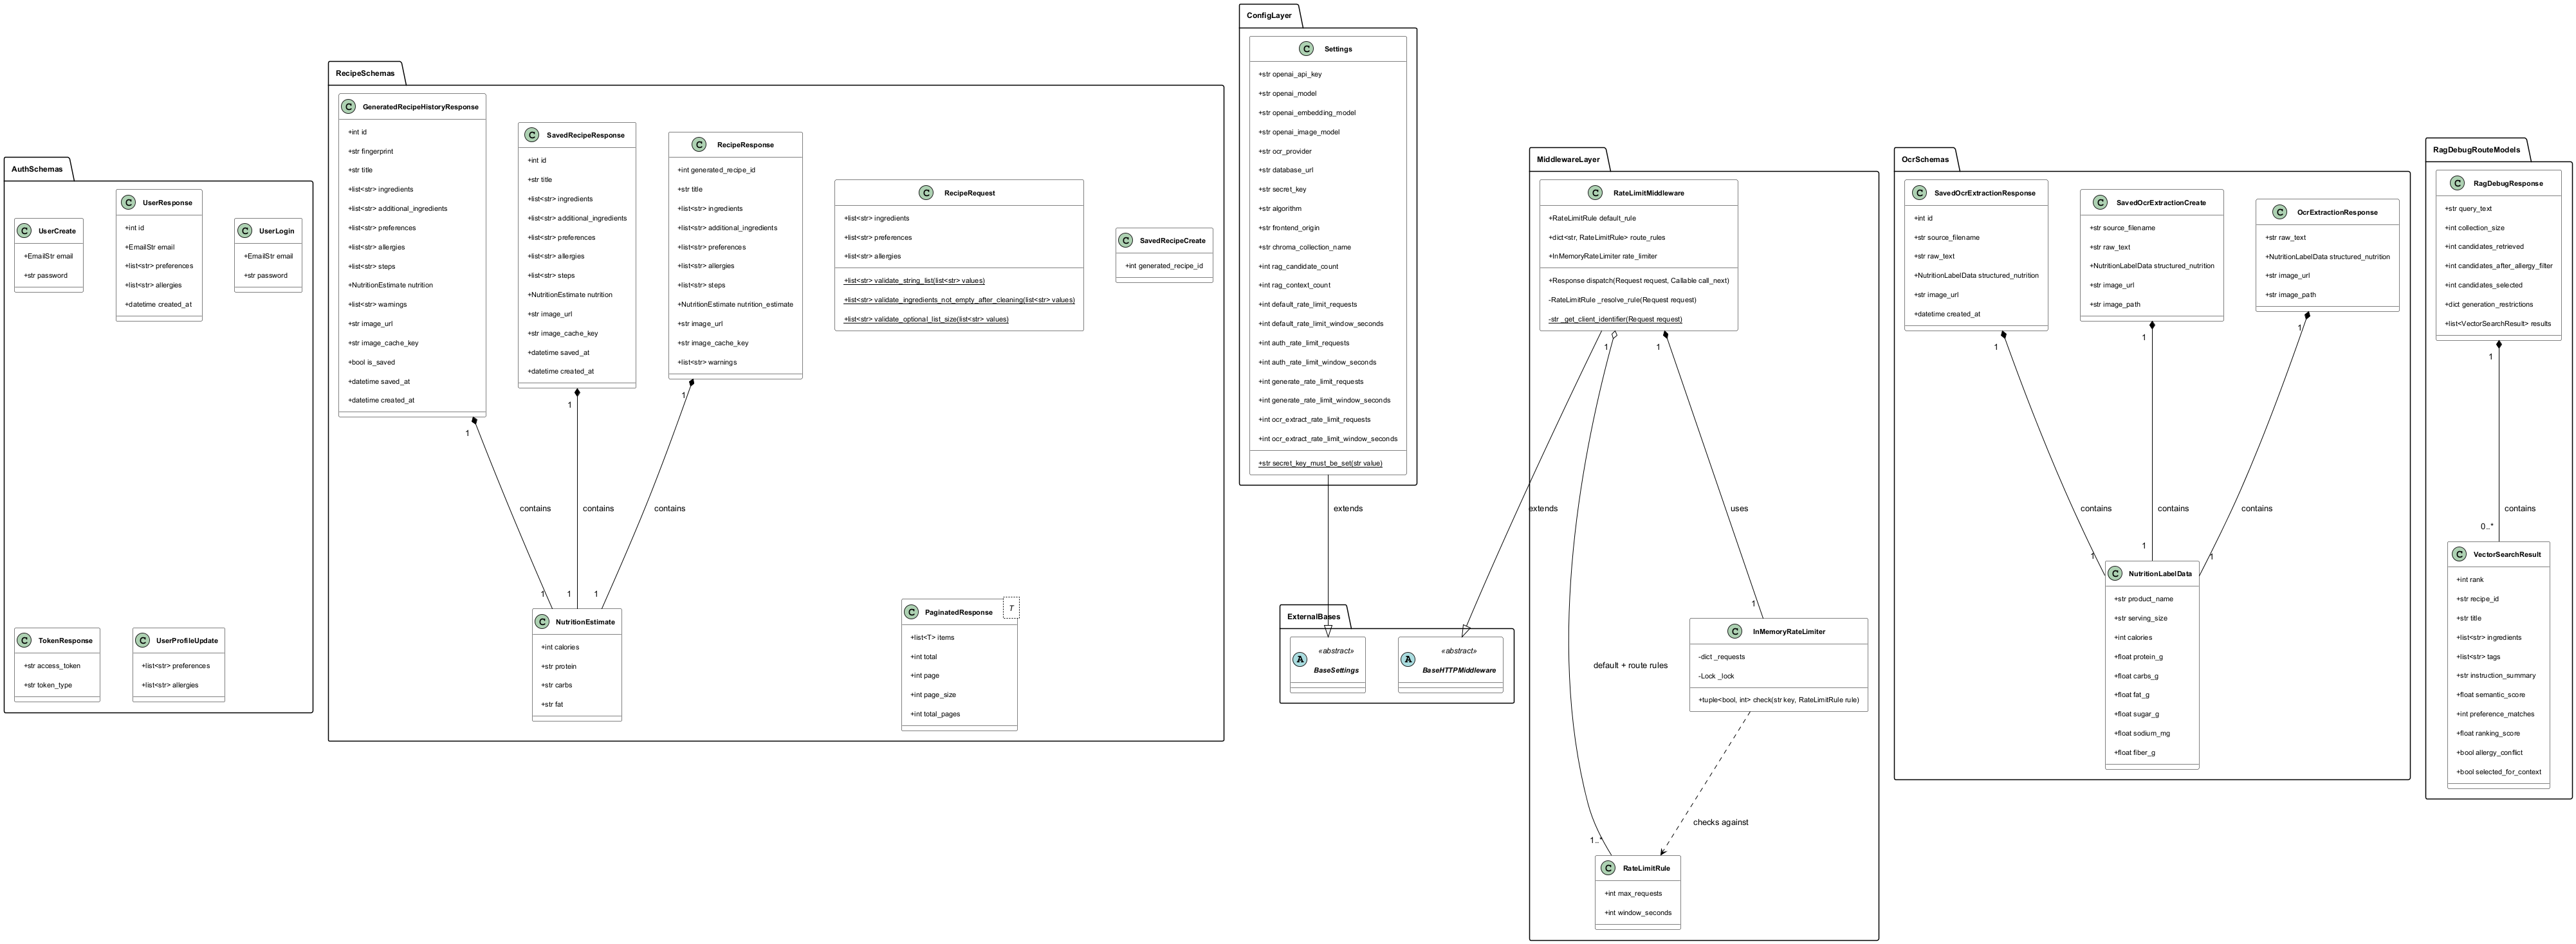
\includegraphics[width=\textwidth]{images/class-diagram-b.png}
	\caption{Class diagram of the infrastructure and schema
	layer, showing API contracts, configuration, middleware,
	and rate-limiting components}
	\label{fig:class-infrastructure}
\end{figure}

These diagrams describe the implemented structure of the system. The
persistent entities correspond to the relational model, the schema
classes define the API boundary, and the provider abstractions separate
vendor-specific OCR and image-generation logic from the rest of the
application. They are mixed on purpose: some parts of the backend are
class-based, while others are clearer as service modules. The diagrams
follow that split instead of pretending that every part of the system
fits one style equally well.

To make this correspondence explicit, Table~\ref{tab:diagram-code-map}
links the main structural artifacts to the implementation units they
describe most directly.

\begin{table}[H]
	\centering
	\scriptsize
	\renewcommand{\arraystretch}{1.2}
	\begin{tabularx}{\textwidth}{|p{2.8cm}|p{4.8cm}|X|}
		\hline
		\textbf{Diagram artifact} & \textbf{Most visible implemented elements} & \textbf{Implementation area} \\
		\hline
		Domain/service class view & \texttt{User}, \texttt{GeneratedRecipe}, \texttt{OcrExtraction}, provider abstractions, route-to-service dependencies & Domain model, recipe workflow services, OCR workflow services, and provider abstractions. \\
		\hline
		Infrastructure/schema class view & \texttt{Settings}, \texttt{RateLimitMiddleware}, \texttt{RateLimitRule}, request and response schemas & Configuration, middleware, and schema-definition modules. \\
		\hline
		Sequence view of recipe generation & Route entry, generation service, retrieval service, provider calls, conditional persistence & Recipe route handling together with retrieval and generation services. \\
		\hline
		State-transition view & Validation, filtering, retrieval, retry, image generation, authenticated persistence & Request validation, recipe orchestration, and thumbnail-generation modules. \\
		\hline
		Use-case and navigation views & User-visible routes and persistence-related page separation & Frontend routing, task pages, and authenticated navigation views. \\
		\hline
		ER and relational views & Entity ownership, nullable vs non-null foreign keys, indexes, and denormalized payload fields & ORM entity definitions and schema-migration history. \\
		\hline
	\end{tabularx}
	\caption{Direct correspondence between the design artifacts and the implementation units}
	\label{tab:diagram-code-map}
\end{table}

\subsubsection{Core workflow design}

The most important backend behavior is not a static entity relation but
a controlled multi-stage workflow. Recipe generation especially benefits
from dynamic modelling because its correctness depends on the order of
operations: validation must happen before retrieval, retrieval before
prompt construction, and output checking before persistence.

The following sequence diagram captures the expected interaction path
for a recipe request. It shows how the frontend, backend route, service
layer, retrieval subsystem, and provider calls cooperate during a single
end-to-end generation.

\begin{figure}[p]
	\centering
	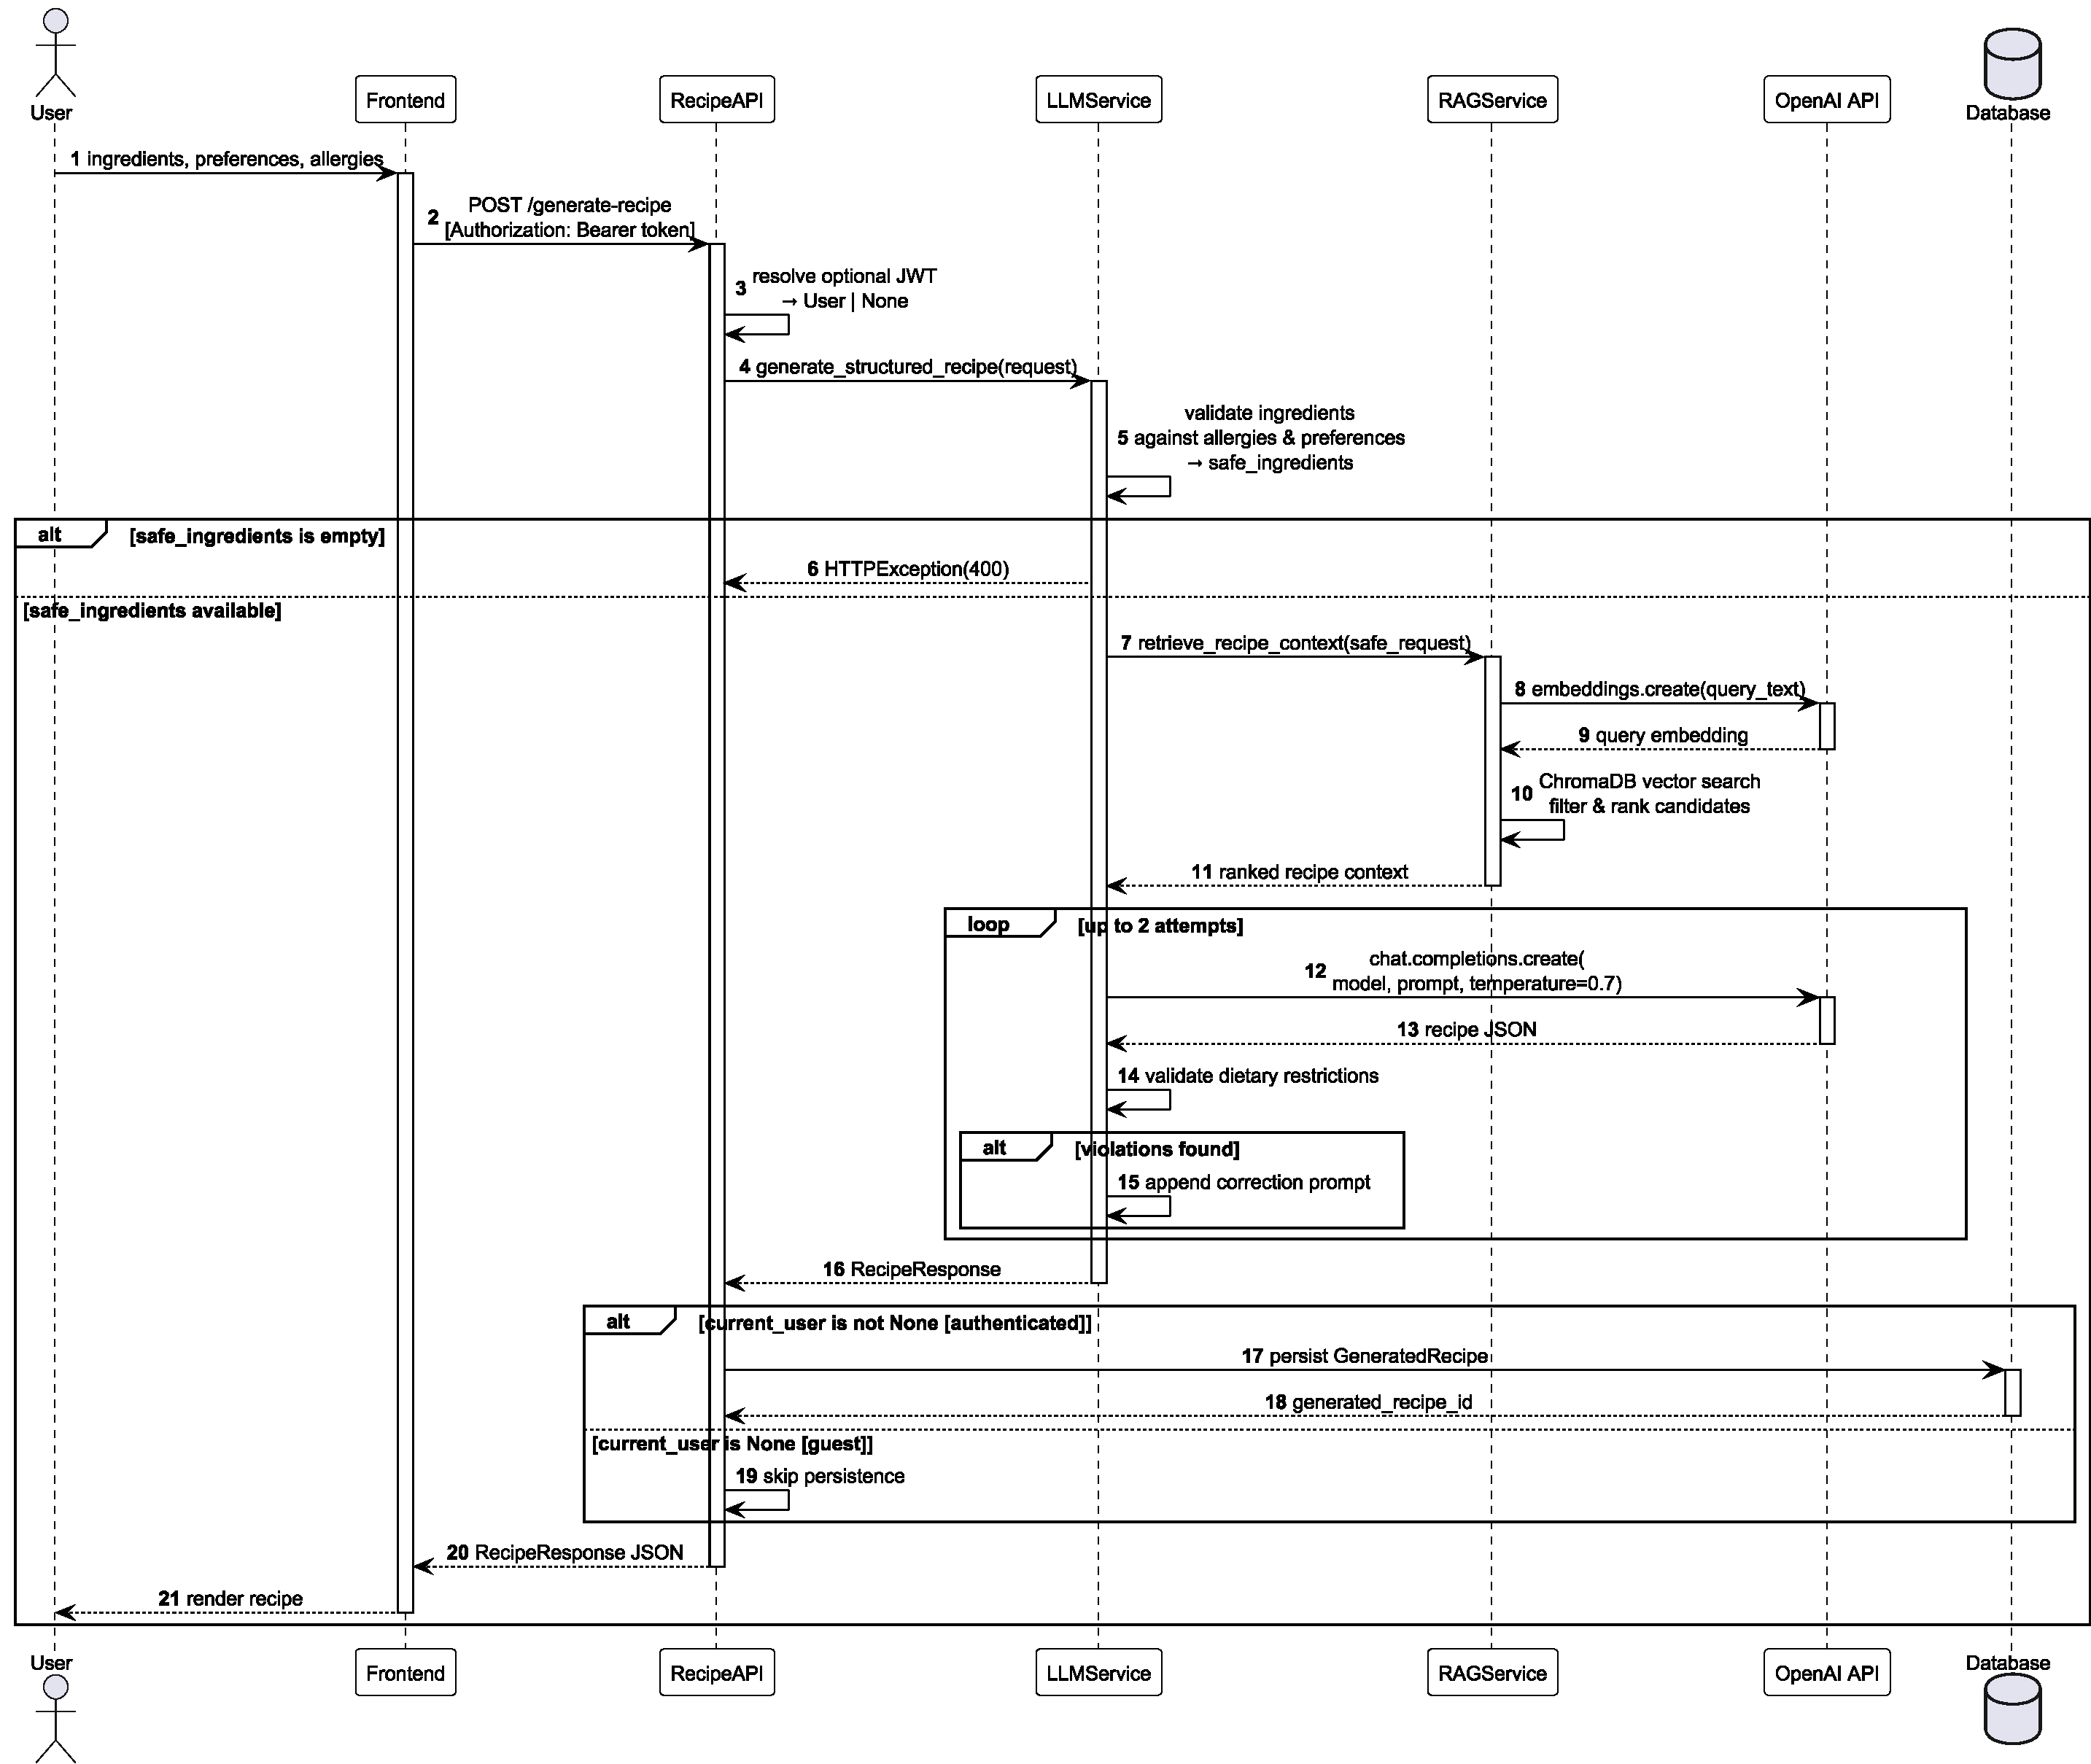
\includegraphics[width=\textwidth]{images/sequence-recipe-generation.pdf}
	\caption{Sequence diagram of the recipe-generation workflow,
	illustrating the call chain from user input through context retrieval,
	LLM invocation, and conditional database persistence}
	\label{fig:design-sequence}
\end{figure}

The sequence view is complemented by a state-oriented and a data-flow
view. The state machine is useful because a recipe request may pass
through correction states before it becomes acceptable, and because
thumbnail generation is intentionally modelled as a non-fatal step. The
data flow diagram is useful because it clarifies which data is produced
or transformed at each stage and which stores participate in the
pipeline. Together, these views document the static structure and the
dynamic behavior of the system from complementary angles.

\begin{figure}[p]
	\centering
	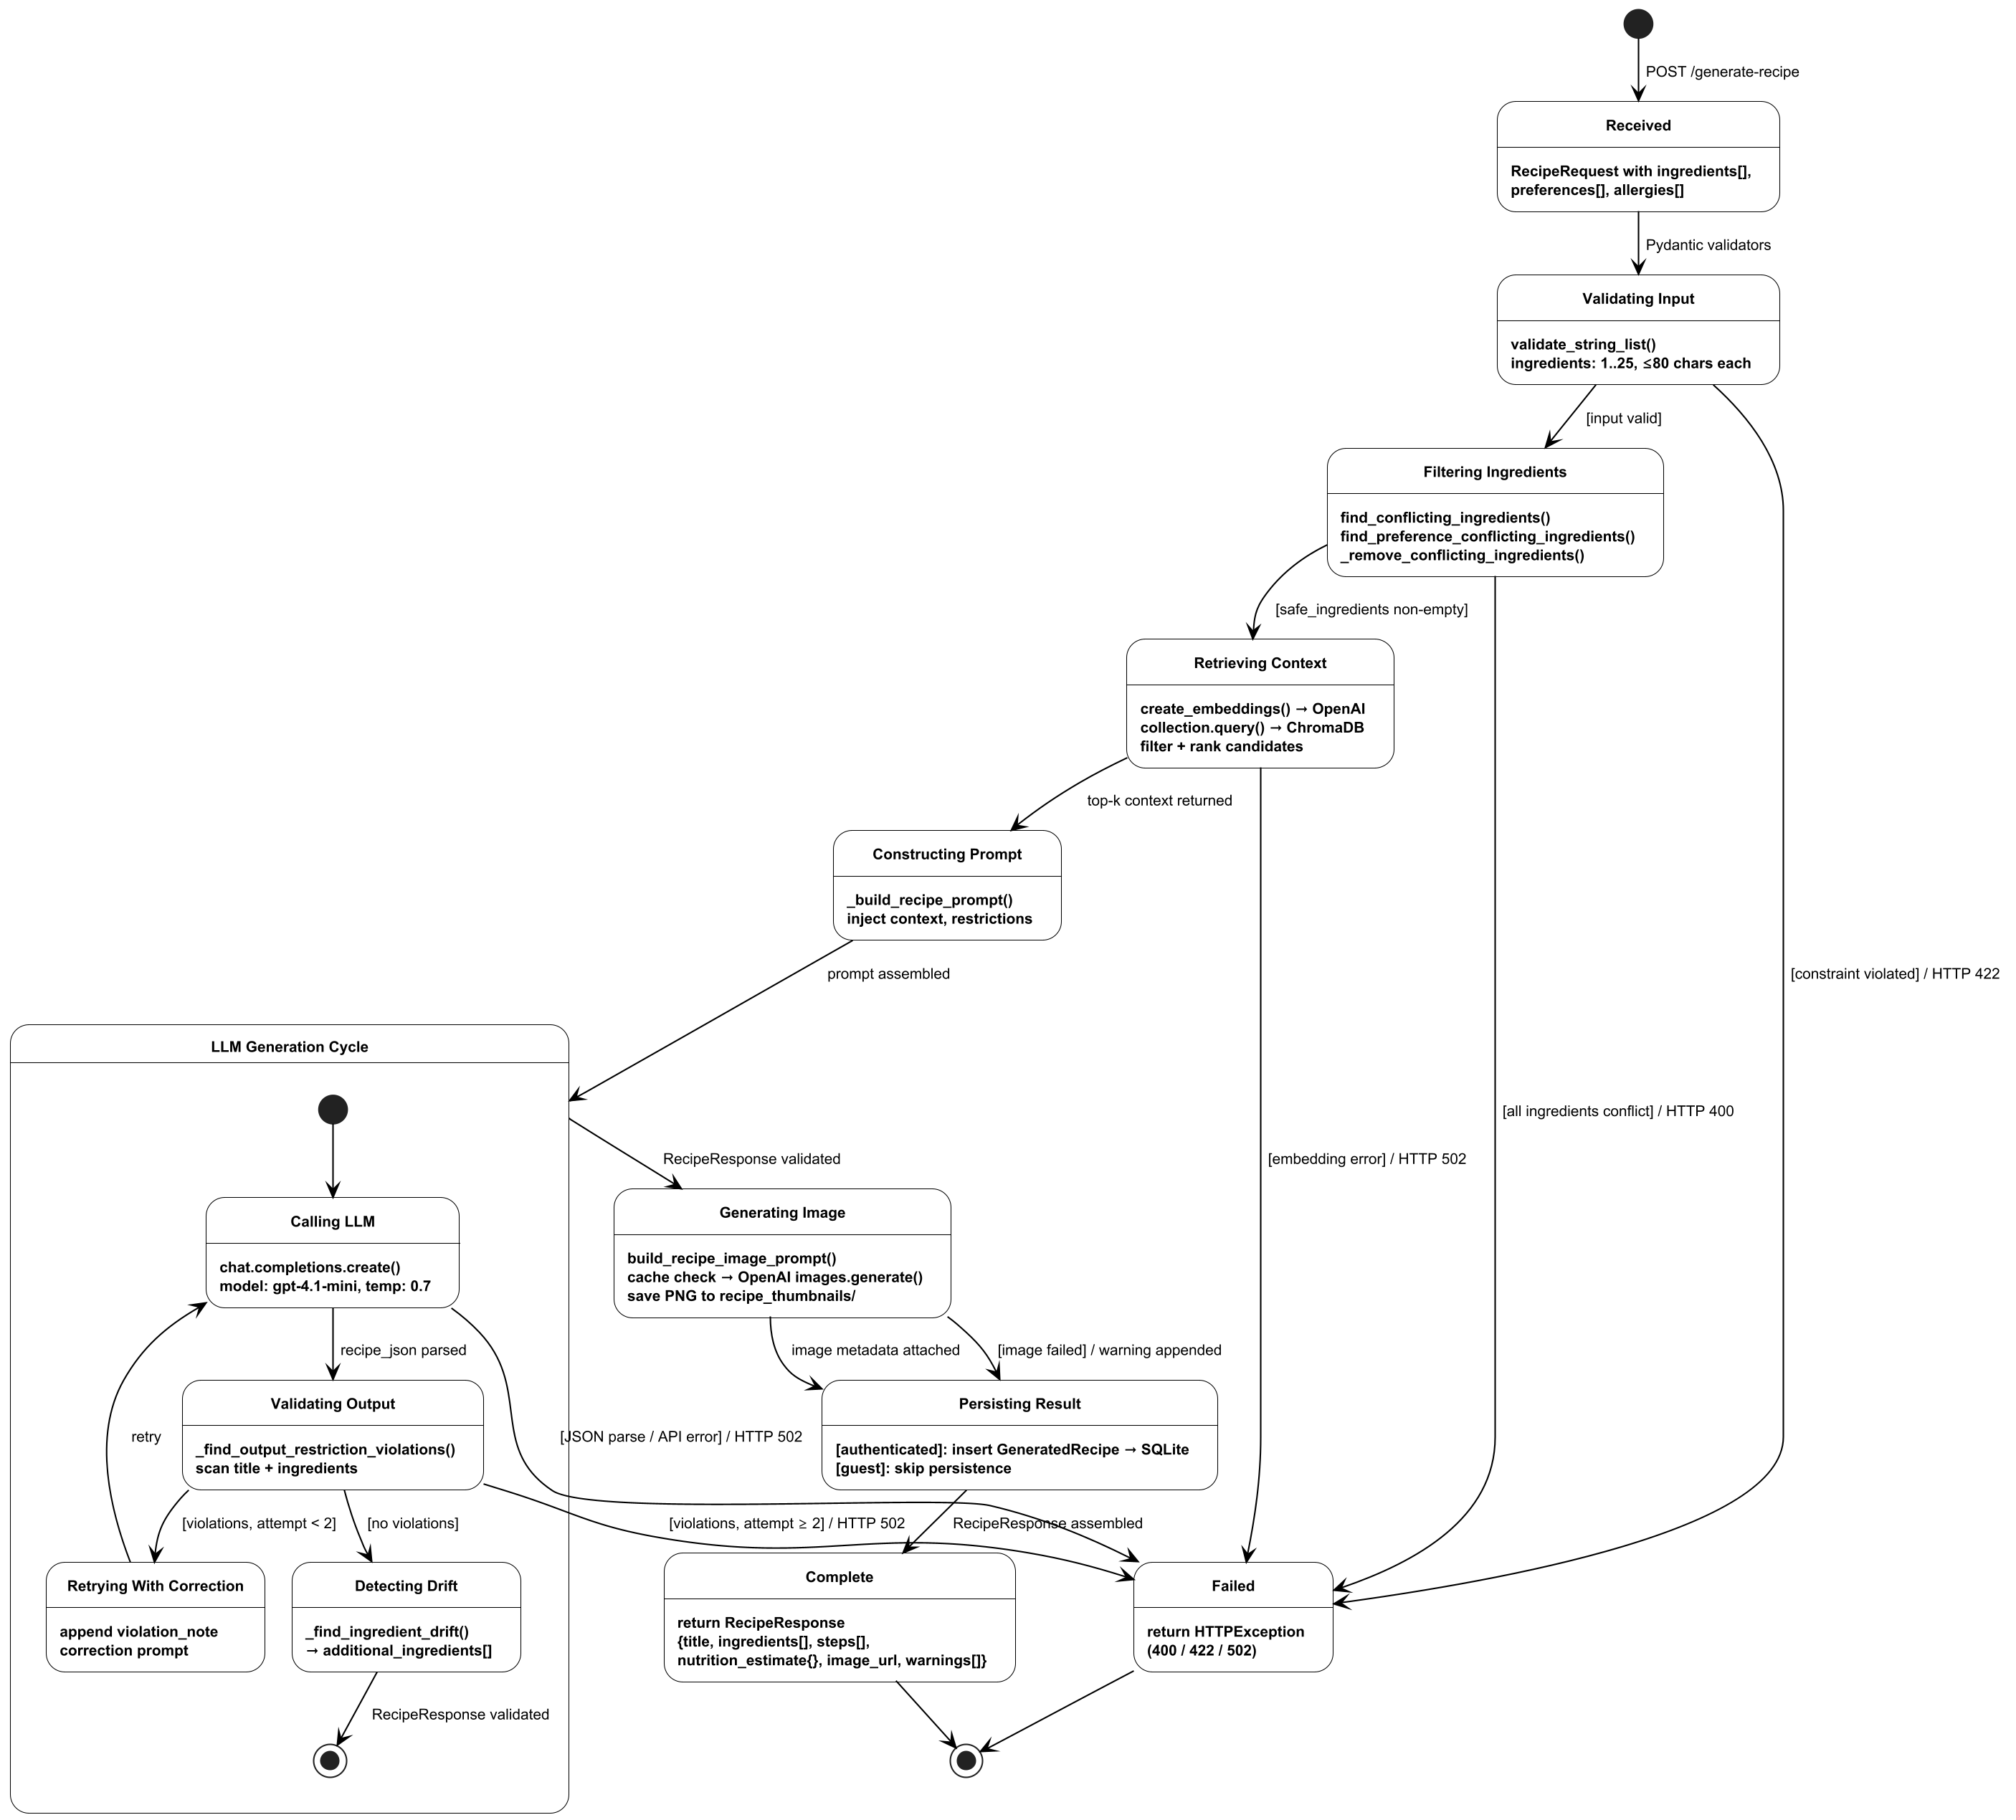
\includegraphics[width=\textwidth,height=0.85\textheight,keepaspectratio]{images/state-transition-recipe-lifecycle.png}
	\caption{State-transition diagram of the recipe request lifecycle,
	showing the path from initial submission through input validation,
	ingredient filtering, retrieval-augmented generation, output
	verification, thumbnail generation, and persistence}
	\label{fig:state-transition}
\end{figure}

\begin{figure}[p]
	\centering
	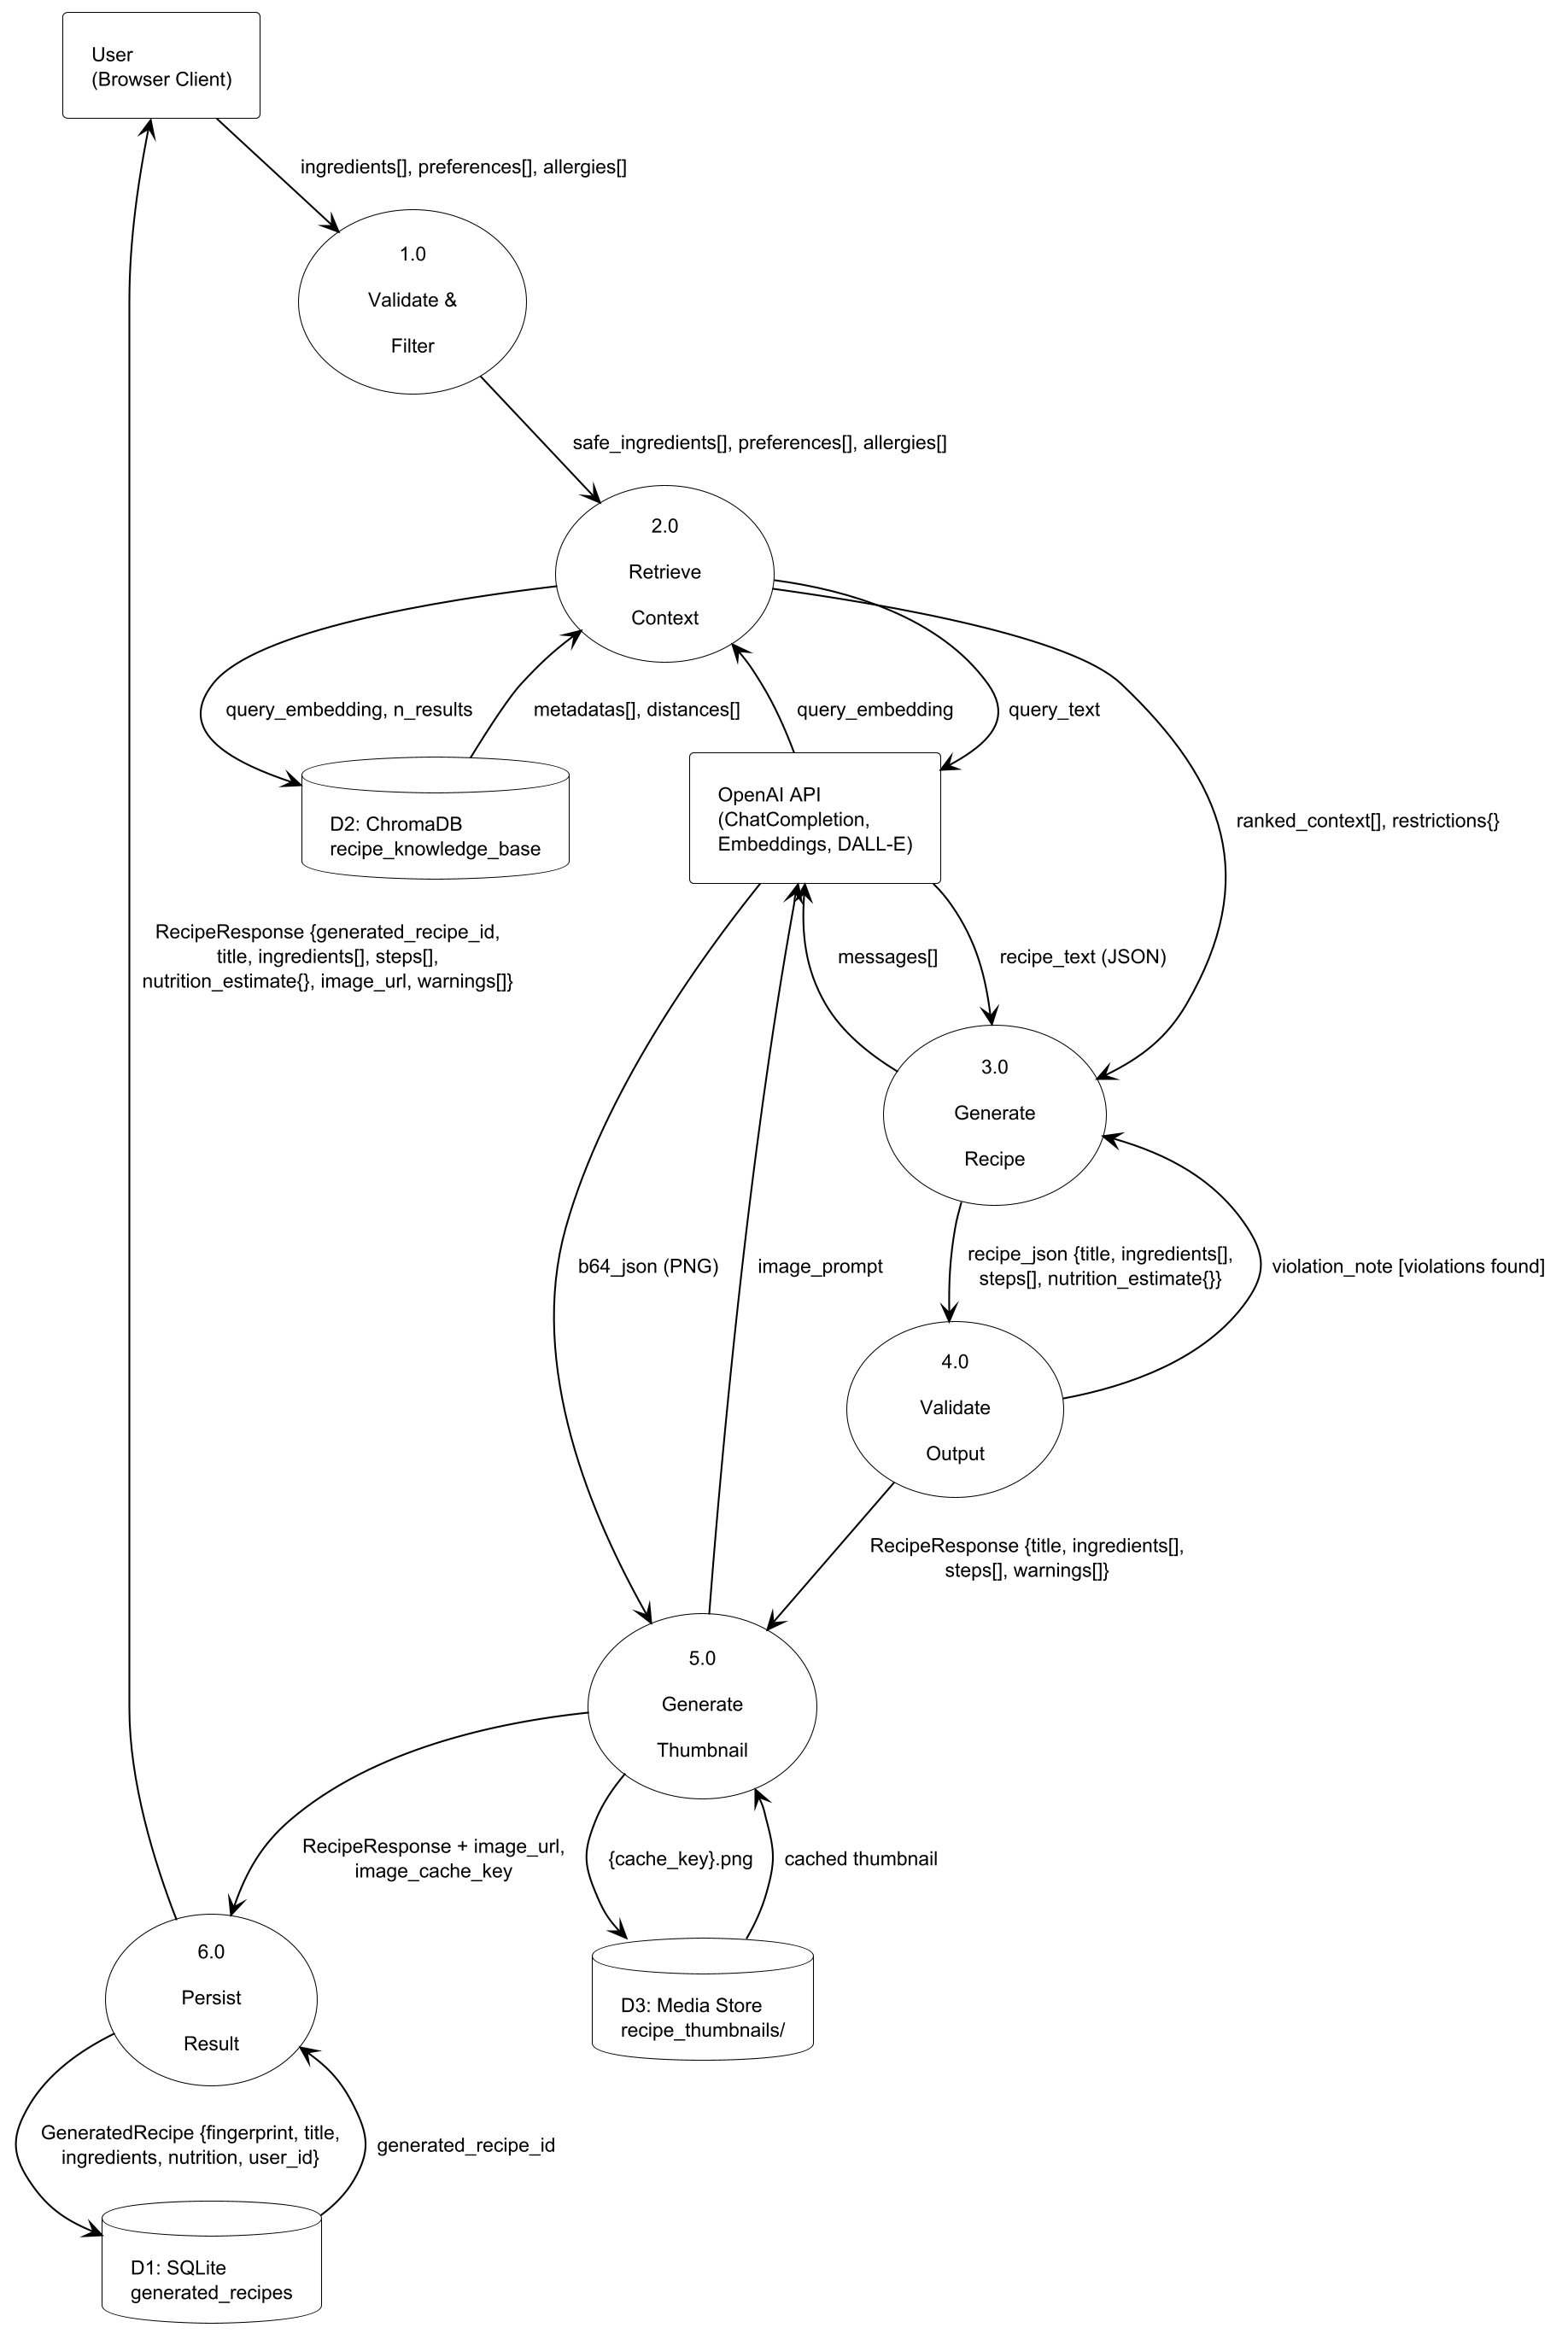
\includegraphics[width=\textwidth,height=0.85\textheight,keepaspectratio]{images/dfd-recipe-generation.png}
	\caption{Level~1 data flow diagram of the recipe-generation
	pipeline, showing processes, data stores, external entities, and
	field-level flows derived from the application codebase}
	\label{fig:dfd}
\end{figure}

Two design decisions are especially important at workflow level.
First, recipe generation is not a single prompt call. The workflow
performs input cleaning, conflict detection, safe-context retrieval,
prompt construction, output validation, optional retry, optional image
generation, and conditional persistence. Second, OCR is explicitly split
into optical extraction and semantic structuring. This separation keeps
failure causes easier to diagnose and allows the OCR provider and the
nutrition-structuring logic to evolve independently.

\subsubsection{API design and interaction model}

The frontend communicates with the backend almost entirely through JSON
API requests. The only exception is OCR upload, where the image itself
is transferred as multipart form data before the backend returns a
structured JSON result. In all cases, the interaction model remains the
same: the frontend sends user input to a dedicated backend route, the
backend validates the request, executes the relevant workflow, and
returns a structured response that the frontend can render directly.

This interaction model keeps the frontend simple. Each page only needs
to know which route to call and what response structure to expect. The
backend remains responsible for authentication, ownership checks,
workflow order, provider calls, and persistence.

\begin{table}[H]
	\centering
	\scriptsize
	\begin{tabular}{|p{2.8cm}|p{11.1cm}|}
		\hline
		\textbf{API area} & \textbf{Purpose and example responsibilities} \\
		\hline
		Authentication API & Supports signup, login, token issuance, current-user retrieval, and profile-default updates. Protected profile operations require authentication and always operate on the resolved current user rather than on client-supplied ownership identifiers. \\
		\hline
		Recipe API & Accepts recipe-generation requests, returns structured recipes with warnings and optional image metadata, persists generated history for authenticated users, and exposes saved-recipe and full-history listings filtered by the authenticated owner. \\
		\hline
		OCR API & Accepts nutrition-label uploads, validates image payloads, returns raw OCR text together with structured nutrition fields, and allows authenticated users to save and browse OCR history under their own account scope. \\
		\hline
		Media/static API & Exposes backend-managed OCR uploads and generated thumbnails as static files addressable from frontend result views and history pages. \\
		\hline
	\end{tabular}
	\caption{Main API areas and their responsibilities}
	\label{tab:api-areas}
\end{table}

\subsubsection{Decision transparency and user-visible evidence}

Because the application relies on external AI services, the design does
not hide intermediate evidence or corrective decisions from the user.
Transparency appears in several concrete forms. Recipe generation can
return warning messages when some provided ingredients were excluded,
when the generated result requires additional ingredients, or when
thumbnail generation fails and the recipe is returned without an image.
The OCR workflow displays the raw extracted text and the structured
nutrition interpretation side by side, which allows the user to judge
whether the semantic structuring step remained faithful to the visible
label content.

This transparency is part of making the system usable. OCR and
language-model services can still return imperfect results, so the
application should show what was read directly from the input and what
was inferred later in the workflow.

\subsubsection{Recurring design mechanisms}

The project uses a layered architecture together with a small number of
recurring design mechanisms that appear across multiple modules. This is
a better description of the system than forcing every decision into a
formal pattern taxonomy. The most important structural pressures in the
project are provider substitution, explicit API contracts, workflow
orchestration, and controlled persistence boundaries.

\begin{table}[H]
	\centering
	\scriptsize
	\renewcommand{\arraystretch}{1.2}
	\begin{tabularx}{\textwidth}{|p{2.5cm}|p{3.8cm}|p{3.8cm}|X|}
		\hline
		\textbf{Mechanism} & \textbf{Implemented form} & \textbf{Implementation area} & \textbf{Why it fits the system} \\
		\hline
		Provider substitution & OCR and image-generation interfaces with concrete implementations & Provider abstractions for OCR and recipe-image generation. & External providers can change without forcing route or workflow logic to depend on vendor-specific SDK calls. \\
		\hline
		Centralized provider construction & Backend-owned provider selection and reuse points & Provider setup and service initialization logic. & Route handlers and service code ask for capabilities, not concrete classes, which keeps creation logic out of application flow. \\
		\hline
		SDK adaptation & Thin wrappers around OpenAI and Google Vision calls & Concrete provider adapter modules. & External APIs are translated into application-level operations such as text extraction and image generation. \\
		\hline
		Service orchestration boundary & Route modules delegate non-trivial workflows to narrow service entry points & Route modules and workflow-service modules. & Multi-stage workflows stay reusable and testable instead of being duplicated across endpoints. \\
		\hline
		Validated data contracts & Request and response schemas separated from ORM entities & API schema layer. & API contracts remain explicit, validated, and independent from persistence concerns. \\
		\hline
		Cross-cutting middleware & Shared rate-limiting and CORS configuration installed at bootstrap time & Application bootstrap and middleware configuration. & Concerns that apply to many routes are kept out of endpoint logic and enforced uniformly. \\
		\hline
	\end{tabularx}
	\caption{Recurring design mechanisms used throughout the system}
	\label{tab:design-patterns}
\end{table}

These decisions matter mainly for maintainability. Route handlers do not
need to know how provider authentication works or how OCR and image
payloads are encoded; they rely on service or provider interfaces.
Likewise, the frontend depends on API contracts instead of the database
schema. That separation is useful in this project because recipe
generation, OCR, retrieval, and persistence all meet in the same
application. Some parts are best described through classes and
relationships, while others are better described as step-by-step
workflows, and the design chapter follows that same split.

\subsection{Data Design}

\subsubsection{Storage responsibilities}

The system uses three forms of storage because the data has three
different roles:

\begin{itemize}
	\item \textbf{Relational storage} for users and historical user data.
	\item \textbf{Vector storage} for recipe-context retrieval.
	\item \textbf{Filesystem storage} for OCR upload images and generated
	thumbnails.
\end{itemize}

This storage split follows the way the application actually uses data.
User accounts and ownership relations fit a relational model. Retrieval
needs embeddings and similarity search. Uploaded images and thumbnails
are easiest to keep as files referenced from the application data.
The dynamic behavior around recipe generation is documented earlier
through the sequence, state-transition, and data-flow diagrams in
Section~3.2, because the non-trivial data transformations in this
project arise from workflow execution rather than from the static
relational model alone.

\subsubsection{Entity--relationship model}

The relational core of the system contains three entities:
\texttt{User}, \texttt{GeneratedRecipe}, and \texttt{OcrExtraction}.

\begin{itemize}
	\item A \texttt{User} stores identity and profile-default information.
	\item A \texttt{GeneratedRecipe} stores the result of a recipe
	generation request and whether the result was explicitly saved.
	\item An \texttt{OcrExtraction} stores the result of a nutrition-label
	extraction associated with a user.
\end{itemize}

The entity relationships are intentionally simple, because the main
complexity of the application lies in workflow logic rather than in a
large relational domain model:

\begin{itemize}
	\item one user may have many generated recipes,
	\item one user may have many OCR extractions,
	\item each generated recipe belongs to at most one user,
	\item each OCR extraction belongs to exactly one user.
\end{itemize}

\begin{figure}[H]
	\centering
	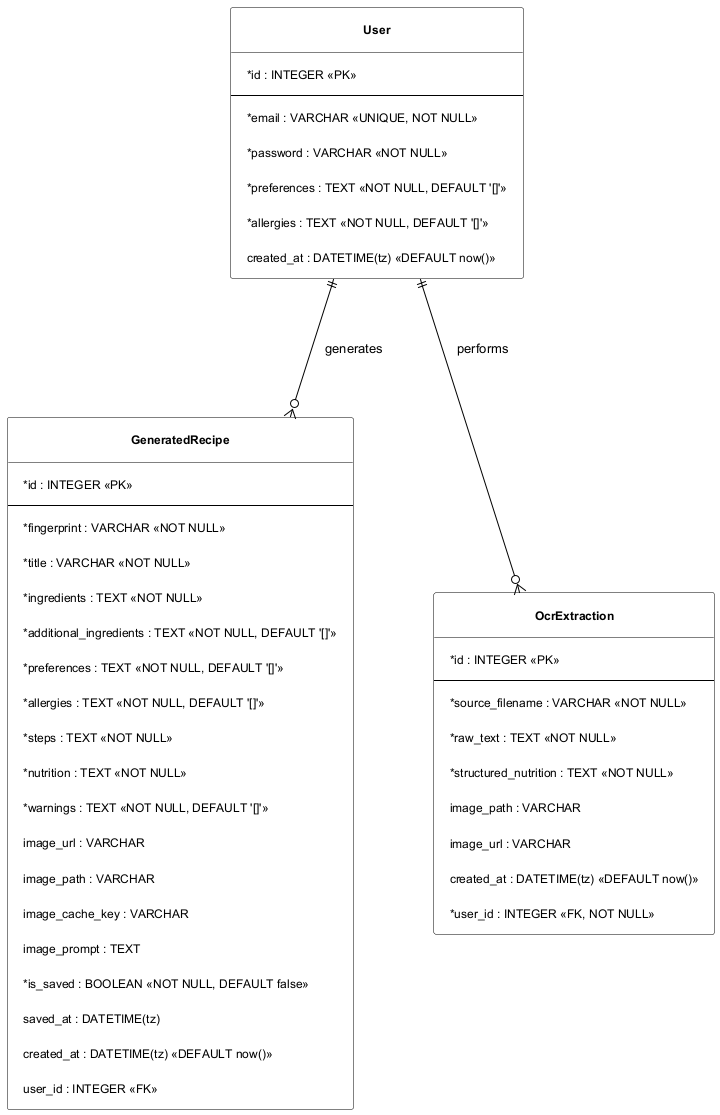
\includegraphics[width=\textwidth]{images/er-diagram.png}
	\caption{Entity-relationship diagram of the AI Cookbook system
	database, showing all entities, attributes, primary keys,
	foreign keys, and cardinality constraints}
	\label{fig:design-erd}
\end{figure}

\subsubsection{Derived relational schema}

From the ER model, the relational schema is derived as shown in
Figure~\ref{fig:relational-schema}. Every table is presented with its
complete column set, data types, key markers, integrity constraints, and
index definitions. The diagram makes the transformation from conceptual
entities to implementable tables explicit, which is important because
the application uses ORM classes but still relies on a concrete
relational design underneath.

The transformation from conceptual model to relational model is direct.
The \texttt{User} entity becomes the \texttt{users} table, the
\texttt{GeneratedRecipe} entity becomes the
\texttt{generated\_recipes} table, and the \texttt{OcrExtraction}
entity becomes the \texttt{ocr\_extractions} table. The two
one-to-many relationships from \texttt{User} are realized by the
\texttt{user\_id} foreign keys in \texttt{generated\_recipes} and
\texttt{ocr\_extractions}. In other words, the ER cardinality ``one
user may own many generated recipes'' is implemented as many rows in
\texttt{generated\_recipes} referencing one row in \texttt{users}, and
the same transformation is used for OCR history.

One detail deserves explicit mention. The
\texttt{generated\_recipes.user\_id} column is nullable at schema level.
This comes from the guest-generation flow, not from a different
ownership rule. The application allows guests to generate recipes, but
only authenticated users can persist them. Keeping the foreign key
nullable makes the schema compatible with that flow, while the
application logic still decides when persistence is allowed. By
contrast, \texttt{ocr\_extractions.user\_id} is non-null because OCR
history entries are created only through an authenticated save action.

\begin{figure}[H]
	\centering
	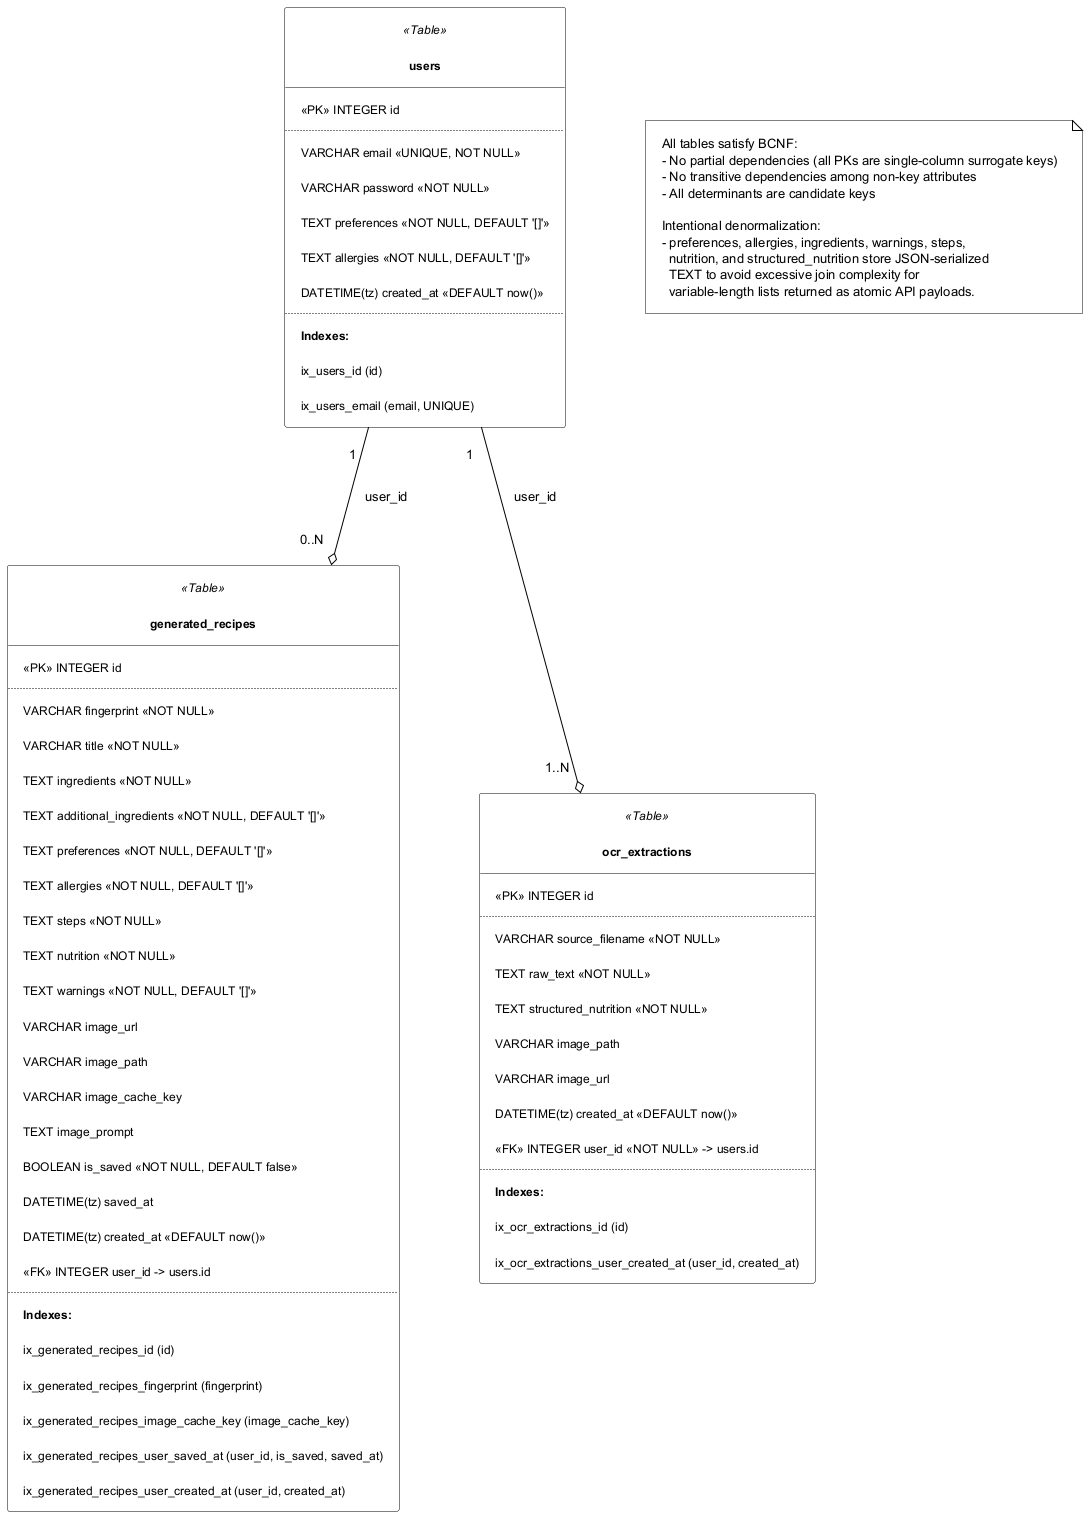
\includegraphics[width=\textwidth]{images/relational-schema.png}
	\caption{Relational schema derived from the ER model, showing all
	tables with primary keys, foreign keys, constraints, indexes, and
	inter-table relationships}
	\label{fig:relational-schema}
\end{figure}

\subsubsection{Normalization analysis}

The database schema of the AI Cookbook system consists of three
relations: \texttt{users}, \texttt{generated\_recipes}, and
\texttt{ocr\_extractions}. Each relation uses a single-column
surrogate integer primary key (\texttt{id}), which makes partial
dependencies structurally impossible and keeps ownership relations easy
to express through foreign keys.

At the relational level, the schema satisfies the usual normalization
requirements up to BCNF. The tables do not contain repeating groups,
their non-key attributes depend on the whole primary key, and there are
no transitive dependencies in which one non-key attribute determines
another. The strongest project-specific example is \texttt{users}: the
unique \texttt{email} attribute supports authentication lookup, while
\texttt{password}, \texttt{preferences}, \texttt{allergies}, and
\texttt{created\_at} all remain directly dependent on the row identity.
The same reasoning applies to \texttt{generated\_recipes} and
\texttt{ocr\_extractions}, where \texttt{user\_id} expresses ownership
but does not determine the remaining descriptive attributes of the row.

The schema does contain intentional denormalization in several
\texttt{TEXT} columns that store JSON-serialized arrays or objects
rather than being decomposed into separate child tables.
Specifically, the \texttt{preferences} and \texttt{allergies}
columns in both \texttt{users} and \texttt{generated\_recipes} store
serialized JSON arrays of strings. The \texttt{ingredients},
\texttt{additional\_ingredients}, \texttt{steps}, \texttt{warnings},
and \texttt{nutrition} columns in \texttt{generated\_recipes}, as
well as \texttt{structured\_nutrition} in
\texttt{ocr\_extractions}, similarly store JSON-encoded structured
data. A strictly normalized design would decompose each of these
into separate child relations. However, this denormalization is a
deliberate design choice driven by the application's access patterns:
every API endpoint that retrieves a recipe or extraction returns
these fields as complete JSON structures in a single response, and
the application never filters or aggregates on individual elements
within them at SQL level. Decomposing them would introduce extra join
cost and mapping complexity for every read while providing little
benefit to the actual queries used by the system.

\subsubsection{Index strategy and query design}

The index design reflects the dominant access paths of the application.

\begin{itemize}
	\item A unique index on \texttt{users.email} supports fast lookup
	during registration and login.
	\item An index on \texttt{generated\_recipes.fingerprint} supports
	recipe-result traceability.
	\item An index on \texttt{generated\_recipes.image\_cache\_key}
	supports thumbnail reuse.
	\item A composite index on
	\texttt{generated\_recipes(user\_id, is\_saved, saved\_at)} supports
	the saved-recipes listing query.
	\item A composite index on
	\texttt{generated\_recipes(user\_id, created\_at)} supports recipe
	history pagination.
	\item A composite index on
	\texttt{ocr\_extractions(user\_id, created\_at)} supports OCR history
	pagination.
\end{itemize}

These indexes are justified directly by the route behavior. The
principal query patterns of the system are the following:

\begin{itemize}
	\item \textbf{Authentication lookup:} find a user by unique
	\texttt{email} during registration, login, and JWT resolution.
	\item \textbf{Ownership-scoped recipe save:} find one generated recipe
	by \texttt{id} and \texttt{user\_id} before setting
	\texttt{is\_saved} and \texttt{saved\_at}.
	\item \textbf{Saved-recipe listing:} filter by \texttt{user\_id} and
	\texttt{is\_saved}, then order primarily by \texttt{saved\_at}.
	\item \textbf{Recipe-history listing:} filter by \texttt{user\_id} and
	order by descending \texttt{created\_at}.
	\item \textbf{OCR-history listing:} filter by \texttt{user\_id} and
	order by descending \texttt{created\_at}.
\end{itemize}

Saved recipes are filtered by owner and save state, then ordered by
\texttt{saved\_at} and \texttt{created\_at}. Recipe history and OCR
history are filtered by owner and ordered by descending creation time.
The indexes were chosen from these concrete queries, not added in
advance without a matching access pattern.

\subsubsection{ORM mapping rationale}

The relational model is reflected in the backend through ORM entity
classes. This was preferred over hand-written SQL-only access because
the application repeatedly converts between request schemas, database
objects, and response schemas. Using ORM-mapped entities keeps the
persistent structure close to the application domain and reduces
duplication between route logic and storage definitions. The design
still remains relationally explicit because the ER diagram, relational
schema, and index strategy are documented independently of the ORM
syntax.

\subsubsection{Vector-store design}

The retrieval subsystem stores recipe documents in a persistent vector
collection. Each stored recipe has two design layers:

\begin{itemize}
	\item \textbf{Document text}, which is embedded and used for semantic
	similarity search.
	\item \textbf{Structured metadata}, which stores title, ingredients,
	tags, steps, summary, and source information used after retrieval.
\end{itemize}

This matters because retrieval is not the final result shown to the
user. The vector store supplies context for later generation. Once a
candidate recipe has been retrieved, its metadata becomes just as
important as the similarity score, because filtering, ranking, and
prompt formatting all depend on those fields.

\subsubsection{Media-storage design}

The media layer stores OCR uploads and recipe thumbnails under
backend-managed directories and exposes them through a static route.
This design is intentionally simple because the project focuses on local
deployment and demonstrable workflows. A file-based approach is enough
here because images support the main features, but they are not queried
as central domain objects.

\subsection{UI/UX Design}

\subsubsection{Low-fidelity wireframes}

The wireframes in Figures~\ref{fig:design-wireframes-main}
and~\ref{fig:design-wireframes-secondary} capture the intended screen
composition before the final interface was polished. Their role is to
show page zoning, information hierarchy, and the separation of the main
user tasks, not the final visual details of the implemented interface.
This is especially important in this project because recipe generation,
OCR verification, persistence, and account management are distinct
workflows with different information needs on screen.

\begin{figure}[p]
	\centering
	\begin{subfigure}[t]{0.48\textwidth}
		\centering
		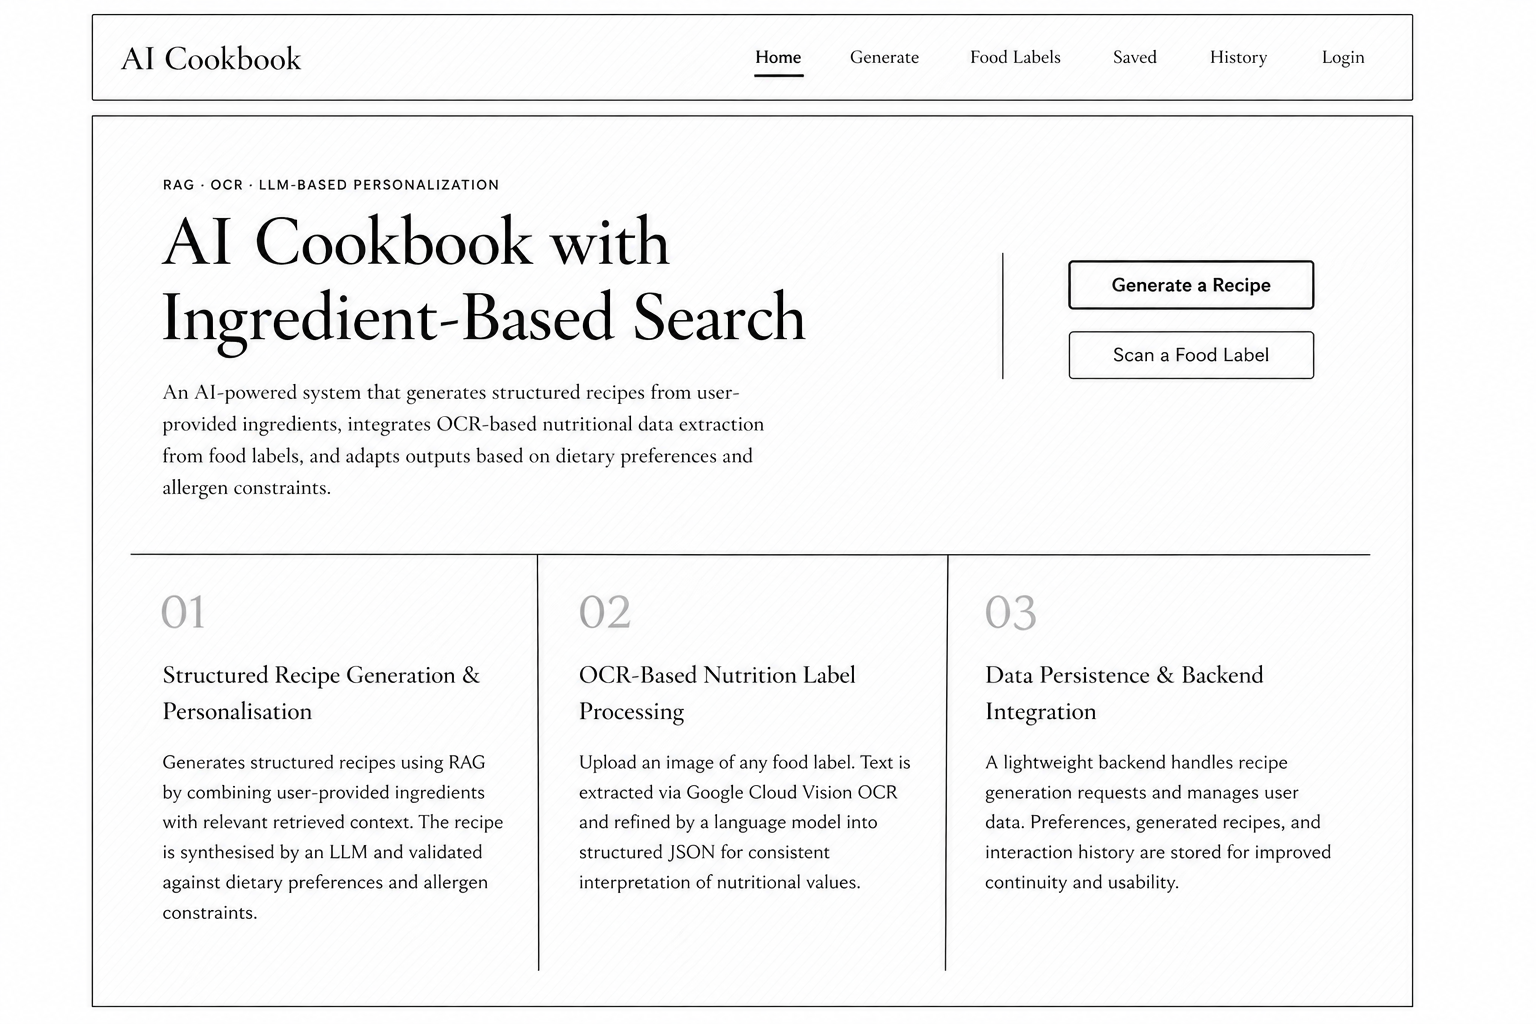
\includegraphics[width=\textwidth]{images/UI/HomeWireframe.png}
		\caption{Home page wireframe}
	\end{subfigure}
	\hfill
	\begin{subfigure}[t]{0.48\textwidth}
		\centering
		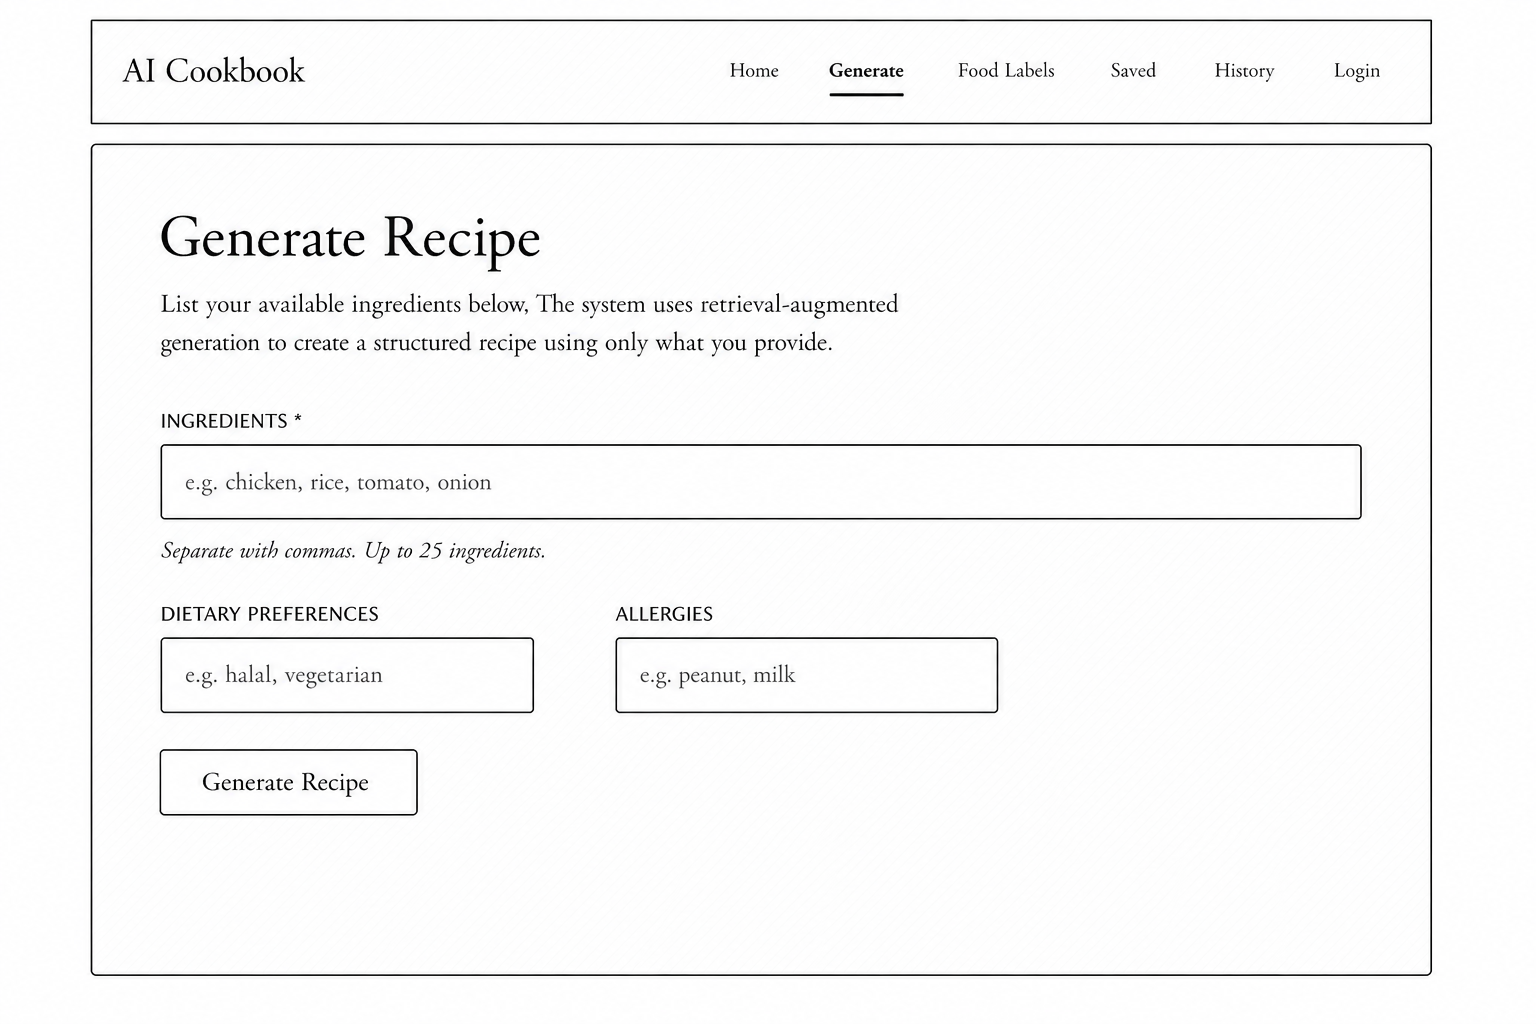
\includegraphics[width=\textwidth]{images/UI/GenerateWireframe.png}
		\caption{Generate page wireframe}
	\end{subfigure}

	\vspace{0.8em}

	\begin{subfigure}[t]{0.48\textwidth}
		\centering
		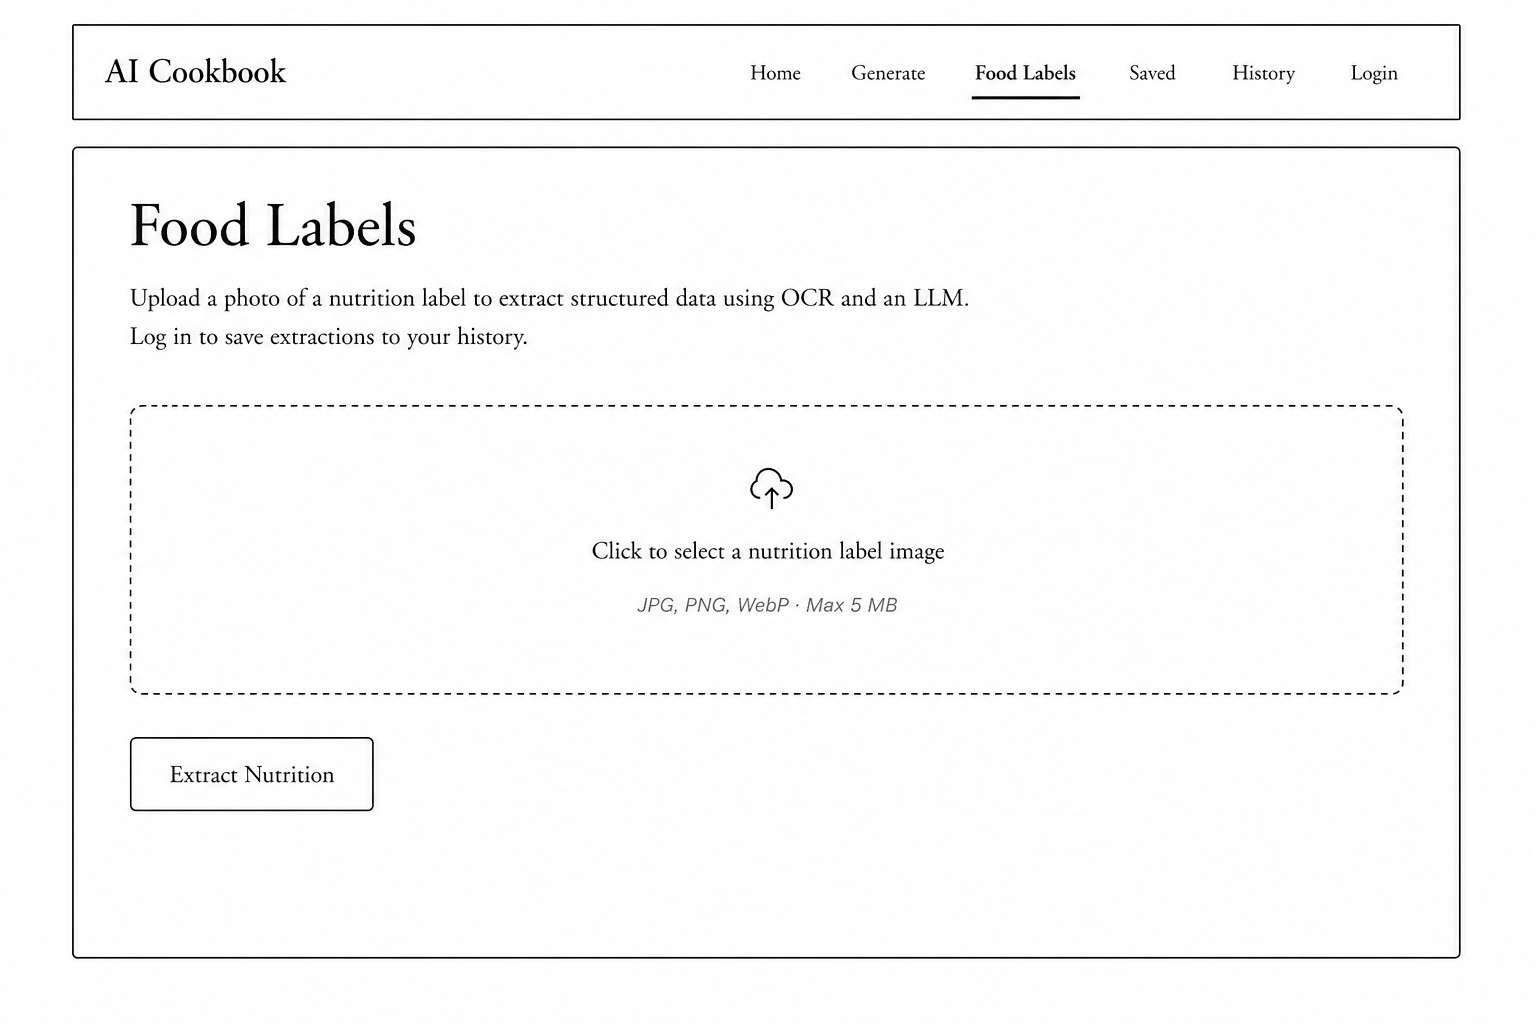
\includegraphics[width=\textwidth]{images/UI/OCRWireframe.png}
		\caption{Food Labels page wireframe}
	\end{subfigure}
	\hfill
	\begin{subfigure}[t]{0.48\textwidth}
		\centering
		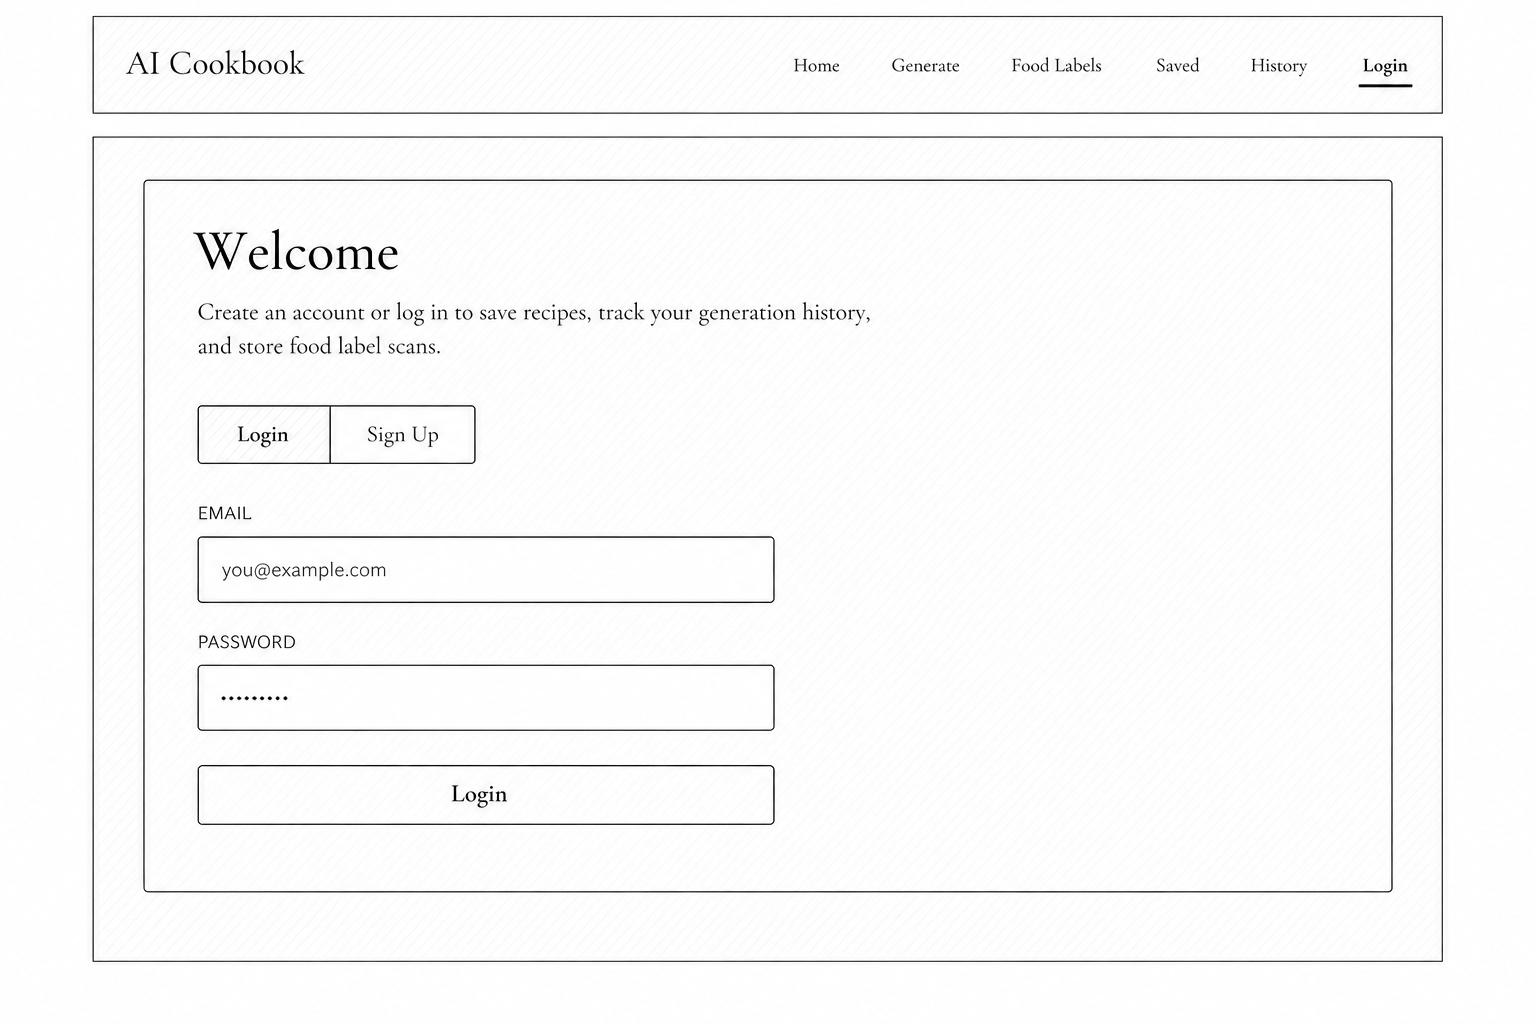
\includegraphics[width=\textwidth]{images/UI/LoginWireframe.png}
		\caption{Login page wireframe}
	\end{subfigure}
	\caption{Primary design-stage wireframes of the main entry and task-oriented pages}
	\label{fig:design-wireframes-main}
\end{figure}

\begin{figure}[p]
	\centering
	\begin{subfigure}[t]{0.48\textwidth}
		\centering
		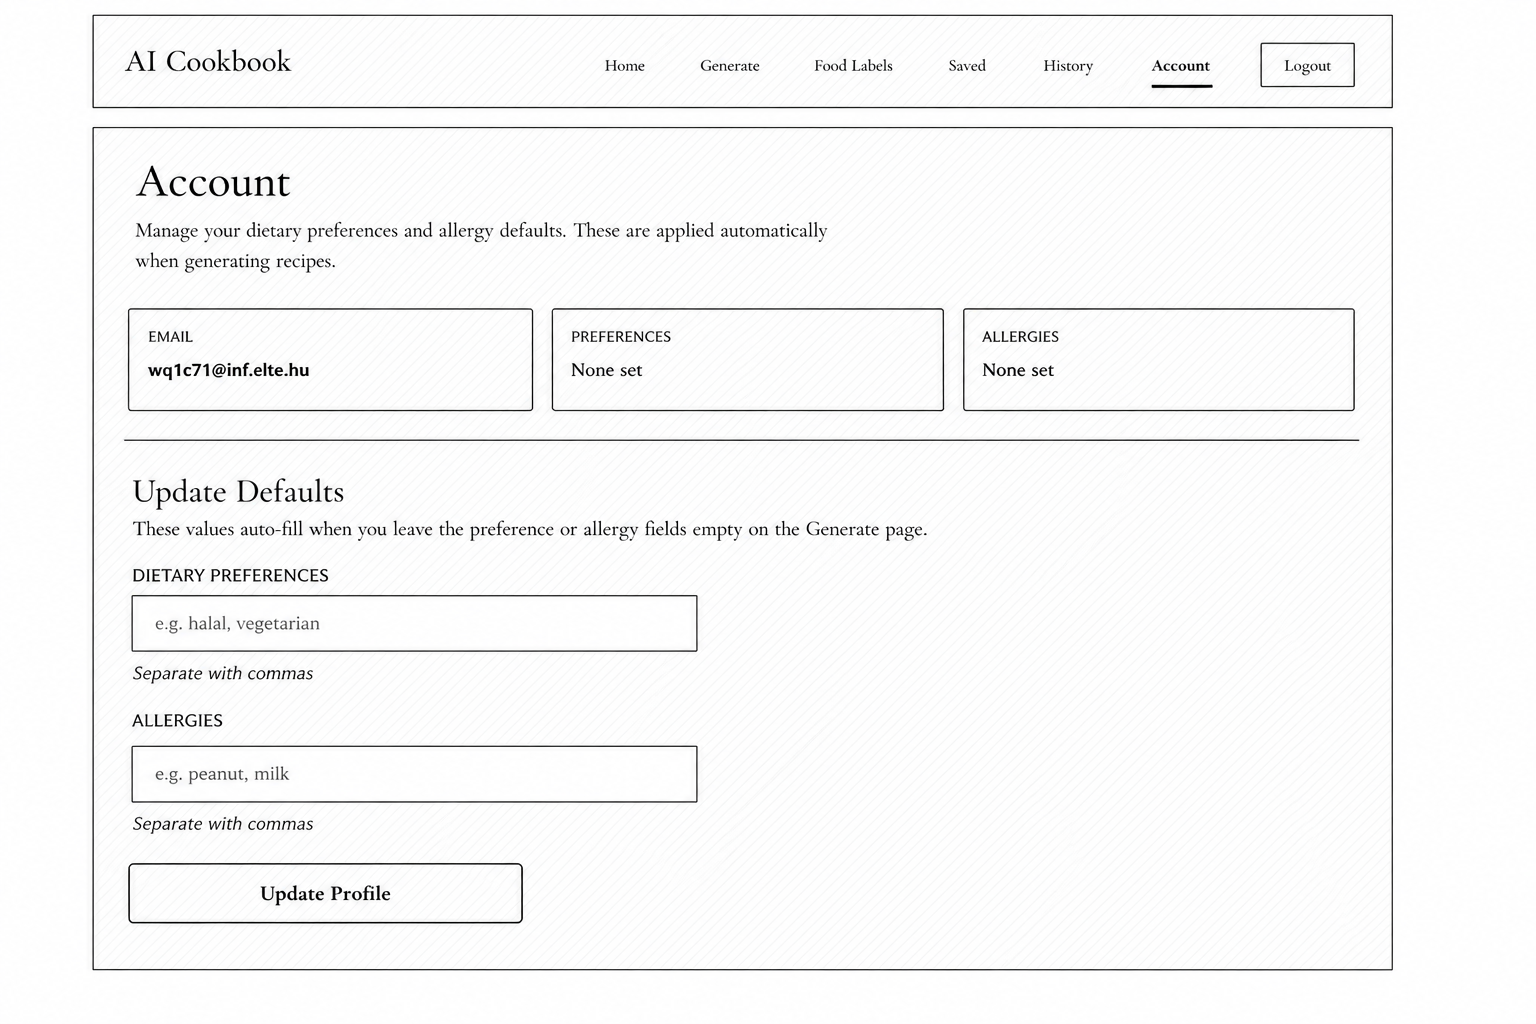
\includegraphics[width=\textwidth]{images/UI/AccountWireframe.png}
		\caption{Account page wireframe}
	\end{subfigure}
	\hfill
	\begin{subfigure}[t]{0.48\textwidth}
		\centering
		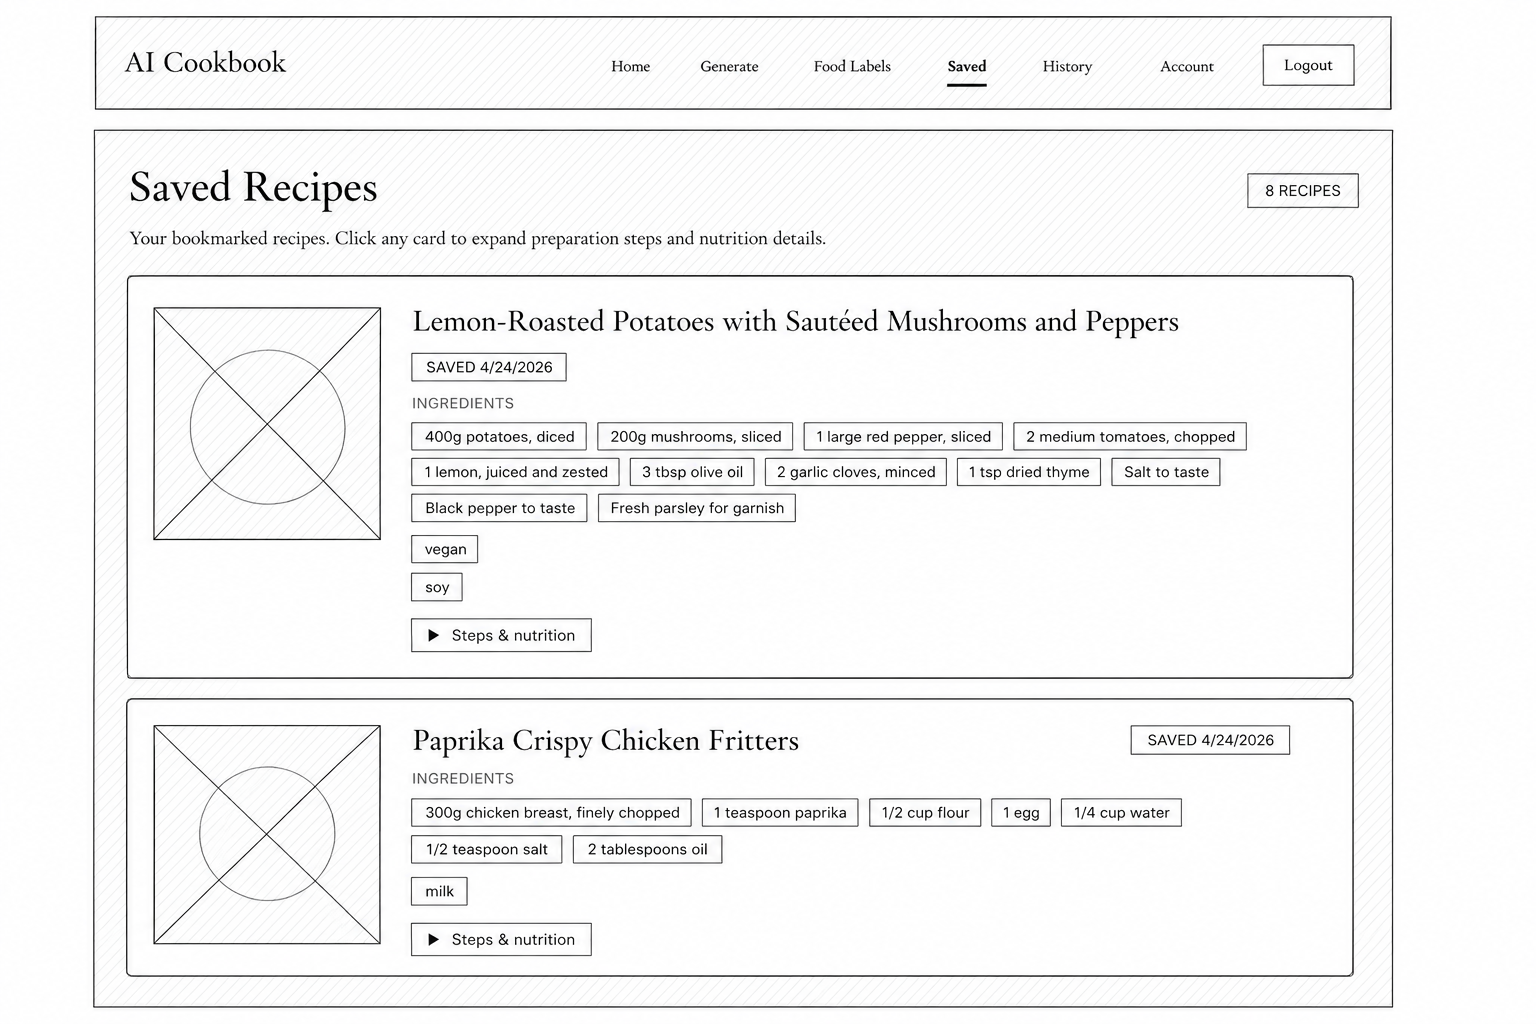
\includegraphics[width=\textwidth]{images/UI/SavedWireframe.png}
		\caption{Saved recipes page wireframe}
	\end{subfigure}

	\vspace{0.8em}

	\begin{subfigure}[t]{0.48\textwidth}
		\centering
		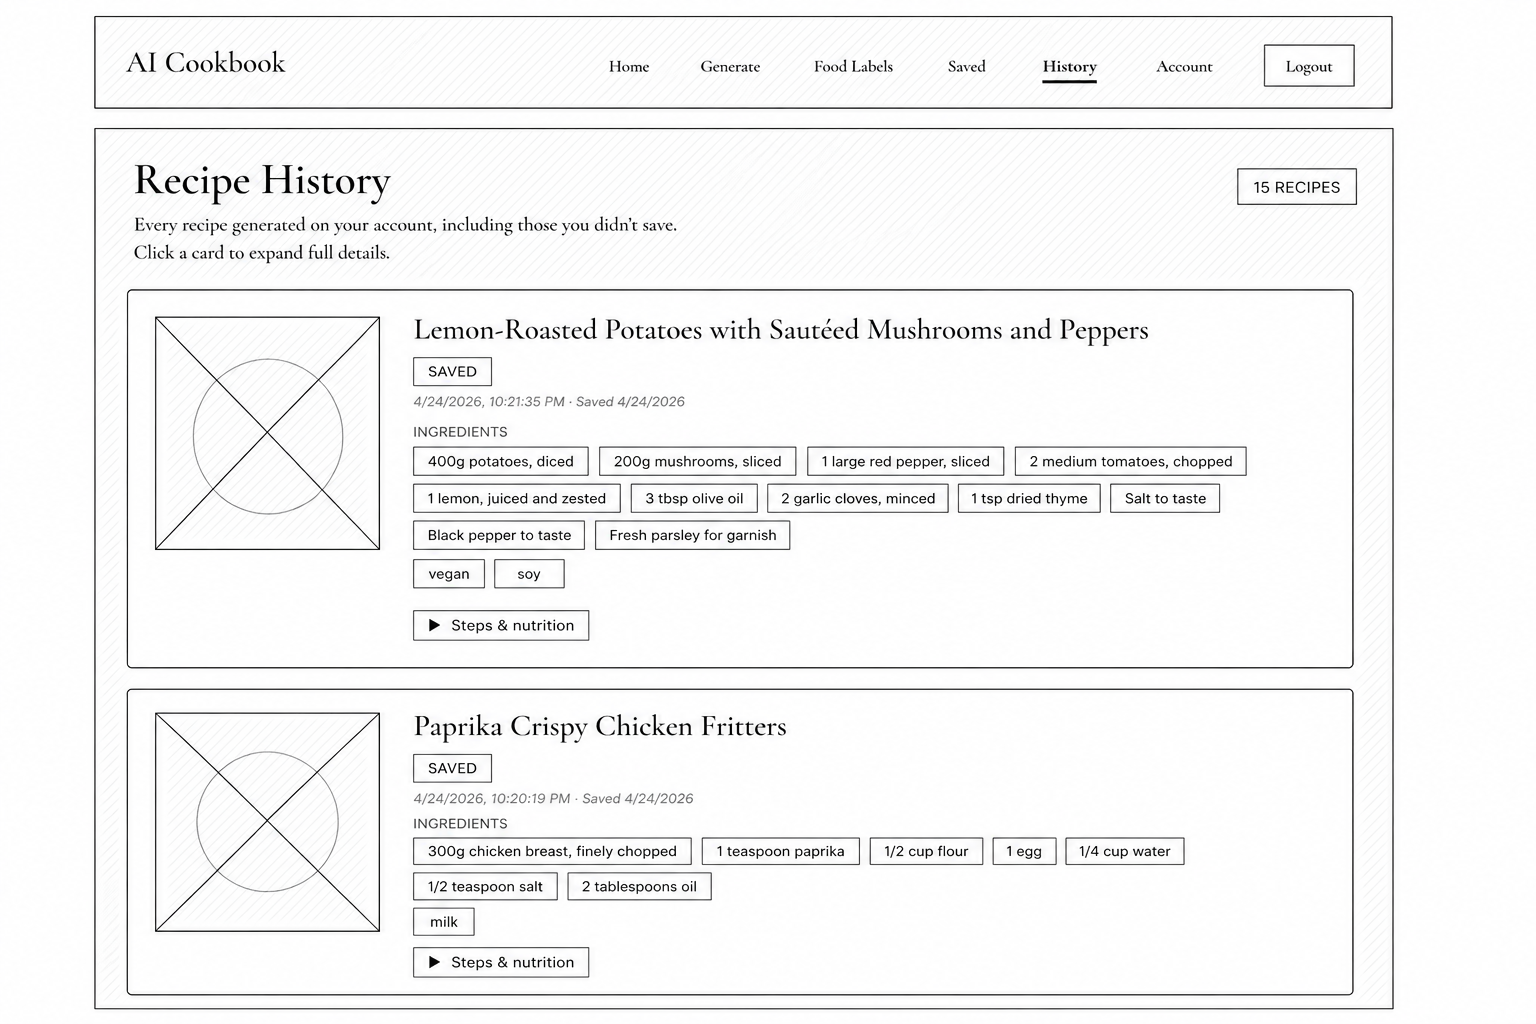
\includegraphics[width=\textwidth]{images/UI/HistoryWireframe.png}
		\caption{History page wireframe}
	\end{subfigure}
	\caption{Secondary design-stage wireframes for persistence and account-related pages}
	\label{fig:design-wireframes-secondary}
\end{figure}

These wireframes already show the three UI decisions that most strongly
influenced the implementation. First, the Generate page reserves space
for dietary constraints near the ingredient input because those
constraints directly shape the generation workflow and warning logic.
Second, recipe warnings deserve a visible zone in the result card
because they communicate safety-relevant information rather than merely
cosmetic status messages. Third, the Food Labels page shows raw OCR text
and the structured nutrition result within the same task view so that
the user can verify how the extraction was interpreted. Finally, save
actions are attached to the result views rather than hidden in secondary
menus, because persistence is a continuation of the primary task rather
than a separate administrative action.

\subsubsection{Navigation structure}

The user interface is organized around a small number of stable routes.
This reduces navigation complexity and makes the main features visible
from the top-level navigation bar.

\begin{itemize}
	\item Home page for overview and entry.
	\item Generate page for recipe-generation tasks.
	\item Food Labels page for OCR extraction tasks.
	\item Saved page for bookmarked recipes.
	\item History page for all generated recipes.
	\item Login / Account page for authentication and default settings.
\end{itemize}

The navigation structure is intentionally task-oriented. Generation,
OCR, persistence, and profile management each have a dedicated visible
location instead of being merged into a single crowded interface.

\subsubsection{Screen-flow design}

\begin{figure}[H]
	\centering
	\resizebox{\textwidth}{!}{
	\begin{tikzpicture}[
		screen/.style={draw, rounded corners, minimum width=3.2cm, minimum height=1.0cm, align=center},
		>=Latex
	]
	\node[screen] (home) at (0,0) {Home};
	\node[screen] (login) at (-4.5,-2.0) {Login / Account};
	\node[screen] (gen) at (0,-2.0) {Generate};
	\node[screen] (ocr) at (4.5,-2.0) {Food Labels};
	\node[screen] (saved) at (-2.2,-4.0) {Saved Recipes};
	\node[screen] (hist) at (2.2,-4.0) {Recipe History};

	\draw[-Latex] (home) -- (login);
	\draw[-Latex] (home) -- (gen);
	\draw[-Latex] (home) -- (ocr);
	\draw[-Latex] (login) -- (gen);
	\draw[-Latex] (login) -- (saved);
	\draw[-Latex] (login) -- (hist);
	\draw[-Latex] (gen) -- (saved);
	\draw[-Latex] (gen) -- (hist);
	\draw[-Latex] (ocr) -- (login);
	\end{tikzpicture}}
	\caption{Navigation and screen-transition map of the main frontend pages}
	\label{fig:design-screen-flow}
\end{figure}

\subsubsection{Interaction design decisions}

Three interaction decisions are especially important at design level.

First, recipe-generation warnings are shown prominently in the result
view because they communicate safety-related information about excluded
ingredients, dietary conflicts, and missing thumbnails.

Second, the OCR page shows both the raw extracted text and the
structured nutrition result. This makes the transformation visible to
the user and supports trust, debugging, and manual verification.

Third, saved recipes and full recipe history are separated into
different pages because they represent different user intentions.
Saved recipes act as a curated personal collection, while history acts
as a chronological activity log.

\subsection{Design alternatives considered}

Several alternative designs were considered, but the final choices were
shaped by the scope of the thesis and by what needed to be implemented
and evaluated clearly.

The first alternative was to use a single-prompt language-model
approach for recipe generation without retrieval grounding. That design
would have been simpler to implement, but it would also have made the
generation process less controllable and less tied to an explicit recipe
knowledge base. Retrieval-augmented generation was chosen because it
creates a stronger connection between user input, reusable corpus
content, and the final prompt while still remaining manageable within
the thesis scope.

The second alternative was to process nutrition labels through one
end-to-end image-to-JSON step. The chosen design instead separates OCR
from semantic structuring. This produces a clearer workflow, supports
debugging through raw OCR text, and makes failure causes easier to
locate when the image-processing and interpretation stages behave
differently.

The third alternative was to use fully cloud-oriented persistence for
the relational database, vector store, and media assets. The project
instead keeps SQLite, Chroma persistence, and local media directories.
This local-storage design is appropriate for a thesis because it keeps
deployment reproducible, reduces infrastructure overhead, and still
demonstrates the architectural responsibilities clearly.

The fourth alternative was to require authentication for every feature.
The chosen guest-plus-authenticated model supports easier exploration of
the main AI-supported workflows while still reserving personal history
and profile persistence for authenticated users. This makes the system
easier to demonstrate and test without weakening the ownership model for
private data.

\subsection{Section Summary}

The design chapter establishes the AI Cookbook as a modular
AI-assisted web application with explicit requirements, a layered
architecture, and a mixed persistence strategy. The use-case,
component, class, sequence, state-transition, data-flow, ER, relational
schema, navigation, and wireframe figures document the system from
complementary viewpoints instead of relying on a single diagram type.

The chapter also makes the project-specific rationale explicit: recipe
generation is implemented as a constrained RAG pipeline rather than as a
single prompt call, OCR is split into optical extraction and semantic
structuring, relational persistence is kept intentionally compact, and
the user interface is organized around a small set of dedicated task
pages. This design forms the basis for the implementation chapter, where
these abstractions are mapped to the final modules and code.
